% Options for packages loaded elsewhere
\PassOptionsToPackage{unicode}{hyperref}
\PassOptionsToPackage{hyphens}{url}
\PassOptionsToPackage{dvipsnames,svgnames,x11names}{xcolor}
%
\documentclass[
  letterpaper,
  DIV=11,
  numbers=noendperiod]{scrartcl}

\usepackage{amsmath,amssymb}
\usepackage{iftex}
\ifPDFTeX
  \usepackage[T1]{fontenc}
  \usepackage[utf8]{inputenc}
  \usepackage{textcomp} % provide euro and other symbols
\else % if luatex or xetex
  \usepackage{unicode-math}
  \defaultfontfeatures{Scale=MatchLowercase}
  \defaultfontfeatures[\rmfamily]{Ligatures=TeX,Scale=1}
\fi
\usepackage{lmodern}
\ifPDFTeX\else  
    % xetex/luatex font selection
\fi
% Use upquote if available, for straight quotes in verbatim environments
\IfFileExists{upquote.sty}{\usepackage{upquote}}{}
\IfFileExists{microtype.sty}{% use microtype if available
  \usepackage[]{microtype}
  \UseMicrotypeSet[protrusion]{basicmath} % disable protrusion for tt fonts
}{}
\makeatletter
\@ifundefined{KOMAClassName}{% if non-KOMA class
  \IfFileExists{parskip.sty}{%
    \usepackage{parskip}
  }{% else
    \setlength{\parindent}{0pt}
    \setlength{\parskip}{6pt plus 2pt minus 1pt}}
}{% if KOMA class
  \KOMAoptions{parskip=half}}
\makeatother
\usepackage{xcolor}
\setlength{\emergencystretch}{3em} % prevent overfull lines
\setcounter{secnumdepth}{-\maxdimen} % remove section numbering
% Make \paragraph and \subparagraph free-standing
\makeatletter
\ifx\paragraph\undefined\else
  \let\oldparagraph\paragraph
  \renewcommand{\paragraph}{
    \@ifstar
      \xxxParagraphStar
      \xxxParagraphNoStar
  }
  \newcommand{\xxxParagraphStar}[1]{\oldparagraph*{#1}\mbox{}}
  \newcommand{\xxxParagraphNoStar}[1]{\oldparagraph{#1}\mbox{}}
\fi
\ifx\subparagraph\undefined\else
  \let\oldsubparagraph\subparagraph
  \renewcommand{\subparagraph}{
    \@ifstar
      \xxxSubParagraphStar
      \xxxSubParagraphNoStar
  }
  \newcommand{\xxxSubParagraphStar}[1]{\oldsubparagraph*{#1}\mbox{}}
  \newcommand{\xxxSubParagraphNoStar}[1]{\oldsubparagraph{#1}\mbox{}}
\fi
\makeatother


\providecommand{\tightlist}{%
  \setlength{\itemsep}{0pt}\setlength{\parskip}{0pt}}\usepackage{longtable,booktabs,array}
\usepackage{calc} % for calculating minipage widths
% Correct order of tables after \paragraph or \subparagraph
\usepackage{etoolbox}
\makeatletter
\patchcmd\longtable{\par}{\if@noskipsec\mbox{}\fi\par}{}{}
\makeatother
% Allow footnotes in longtable head/foot
\IfFileExists{footnotehyper.sty}{\usepackage{footnotehyper}}{\usepackage{footnote}}
\makesavenoteenv{longtable}
\usepackage{graphicx}
\makeatletter
\newsavebox\pandoc@box
\newcommand*\pandocbounded[1]{% scales image to fit in text height/width
  \sbox\pandoc@box{#1}%
  \Gscale@div\@tempa{\textheight}{\dimexpr\ht\pandoc@box+\dp\pandoc@box\relax}%
  \Gscale@div\@tempb{\linewidth}{\wd\pandoc@box}%
  \ifdim\@tempb\p@<\@tempa\p@\let\@tempa\@tempb\fi% select the smaller of both
  \ifdim\@tempa\p@<\p@\scalebox{\@tempa}{\usebox\pandoc@box}%
  \else\usebox{\pandoc@box}%
  \fi%
}
% Set default figure placement to htbp
\def\fps@figure{htbp}
\makeatother
% definitions for citeproc citations
\NewDocumentCommand\citeproctext{}{}
\NewDocumentCommand\citeproc{mm}{%
  \begingroup\def\citeproctext{#2}\cite{#1}\endgroup}
\makeatletter
 % allow citations to break across lines
 \let\@cite@ofmt\@firstofone
 % avoid brackets around text for \cite:
 \def\@biblabel#1{}
 \def\@cite#1#2{{#1\if@tempswa , #2\fi}}
\makeatother
\newlength{\cslhangindent}
\setlength{\cslhangindent}{1.5em}
\newlength{\csllabelwidth}
\setlength{\csllabelwidth}{3em}
\newenvironment{CSLReferences}[2] % #1 hanging-indent, #2 entry-spacing
 {\begin{list}{}{%
  \setlength{\itemindent}{0pt}
  \setlength{\leftmargin}{0pt}
  \setlength{\parsep}{0pt}
  % turn on hanging indent if param 1 is 1
  \ifodd #1
   \setlength{\leftmargin}{\cslhangindent}
   \setlength{\itemindent}{-1\cslhangindent}
  \fi
  % set entry spacing
  \setlength{\itemsep}{#2\baselineskip}}}
 {\end{list}}
\usepackage{calc}
\newcommand{\CSLBlock}[1]{\hfill\break\parbox[t]{\linewidth}{\strut\ignorespaces#1\strut}}
\newcommand{\CSLLeftMargin}[1]{\parbox[t]{\csllabelwidth}{\strut#1\strut}}
\newcommand{\CSLRightInline}[1]{\parbox[t]{\linewidth - \csllabelwidth}{\strut#1\strut}}
\newcommand{\CSLIndent}[1]{\hspace{\cslhangindent}#1}

\KOMAoption{captions}{tableheading}
\makeatletter
\@ifpackageloaded{caption}{}{\usepackage{caption}}
\AtBeginDocument{%
\ifdefined\contentsname
  \renewcommand*\contentsname{Table of contents}
\else
  \newcommand\contentsname{Table of contents}
\fi
\ifdefined\listfigurename
  \renewcommand*\listfigurename{List of Figures}
\else
  \newcommand\listfigurename{List of Figures}
\fi
\ifdefined\listtablename
  \renewcommand*\listtablename{List of Tables}
\else
  \newcommand\listtablename{List of Tables}
\fi
\ifdefined\figurename
  \renewcommand*\figurename{Figure}
\else
  \newcommand\figurename{Figure}
\fi
\ifdefined\tablename
  \renewcommand*\tablename{Table}
\else
  \newcommand\tablename{Table}
\fi
}
\@ifpackageloaded{float}{}{\usepackage{float}}
\floatstyle{ruled}
\@ifundefined{c@chapter}{\newfloat{codelisting}{h}{lop}}{\newfloat{codelisting}{h}{lop}[chapter]}
\floatname{codelisting}{Listing}
\newcommand*\listoflistings{\listof{codelisting}{List of Listings}}
\makeatother
\makeatletter
\makeatother
\makeatletter
\@ifpackageloaded{caption}{}{\usepackage{caption}}
\@ifpackageloaded{subcaption}{}{\usepackage{subcaption}}
\makeatother

\usepackage{bookmark}

\IfFileExists{xurl.sty}{\usepackage{xurl}}{} % add URL line breaks if available
\urlstyle{same} % disable monospaced font for URLs
\hypersetup{
  pdftitle={Foundations of Social, Cognitive, and Affective Neuroscience},
  colorlinks=true,
  linkcolor={blue},
  filecolor={Maroon},
  citecolor={Blue},
  urlcolor={Blue},
  pdfcreator={LaTeX via pandoc}}


\title{Foundations of Social, Cognitive, and Affective Neuroscience}
\usepackage{etoolbox}
\makeatletter
\providecommand{\subtitle}[1]{% add subtitle to \maketitle
  \apptocmd{\@title}{\par {\large #1 \par}}{}{}
}
\makeatother
\subtitle{PSY 511.003 Spr 2025}
\author{}
\date{}

\begin{document}
\maketitle


\section{Overview}\label{overview}

\subsection{Prelude}\label{prelude}

\begin{center}\rule{0.5\linewidth}{0.5pt}\end{center}

\url{https://www.youtube.com/embed/JB7jSFeVz1U}

melodysheep (2011)

\begin{center}\rule{0.5\linewidth}{0.5pt}\end{center}

\begin{quote}
``\emph{If understanding everything we need to know about the brain is a
mile, how far have we walked?}''
\end{quote}

National Geographic (2014)

\begin{center}\rule{0.5\linewidth}{0.5pt}\end{center}

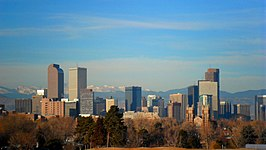
\includegraphics[width=\linewidth,height=1.5625in,keepaspectratio]{img_gilmore_bio/266px-DenverCP.JPG}

\includegraphics[width=\linewidth,height=1.5625in,keepaspectratio]{img_gilmore_bio/brown_large.png}
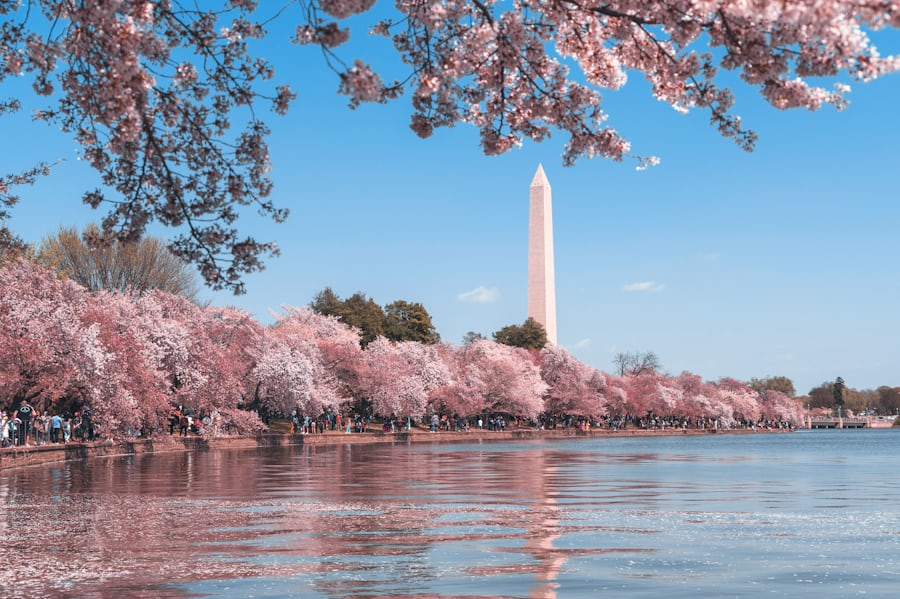
\includegraphics[width=\linewidth,height=1.5625in,keepaspectratio]{img_gilmore_bio/wash-monument.jpeg}


\includegraphics[width=\linewidth,height=1.5625in,keepaspectratio]{img_gilmore_bio/cmu-logo.jpg}

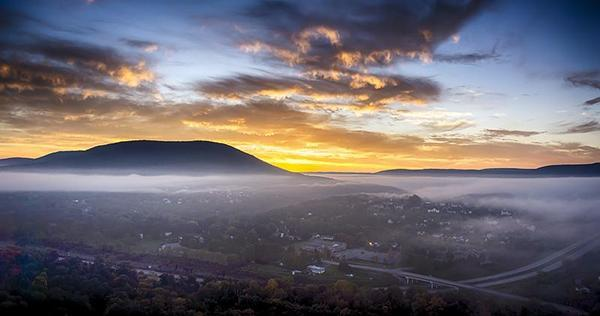
\includegraphics[width=\linewidth,height=1.5625in,keepaspectratio]{img_gilmore_bio/mt-nittany.png}


\includegraphics[width=\linewidth,height=1.5625in,keepaspectratio]{img_gilmore_bio/sleic.png}

\begin{center}\rule{0.5\linewidth}{0.5pt}\end{center}

\begin{center}

\includegraphics[width=\linewidth,height=1.5625in,keepaspectratio]{../include/img/databrary-nav.png}
\end{center}
\begin{center}

\includegraphics[width=\linewidth,height=1.5625in,keepaspectratio]{img_gilmore_bio/PLAY-logo.png}
\end{center}
\begin{center}
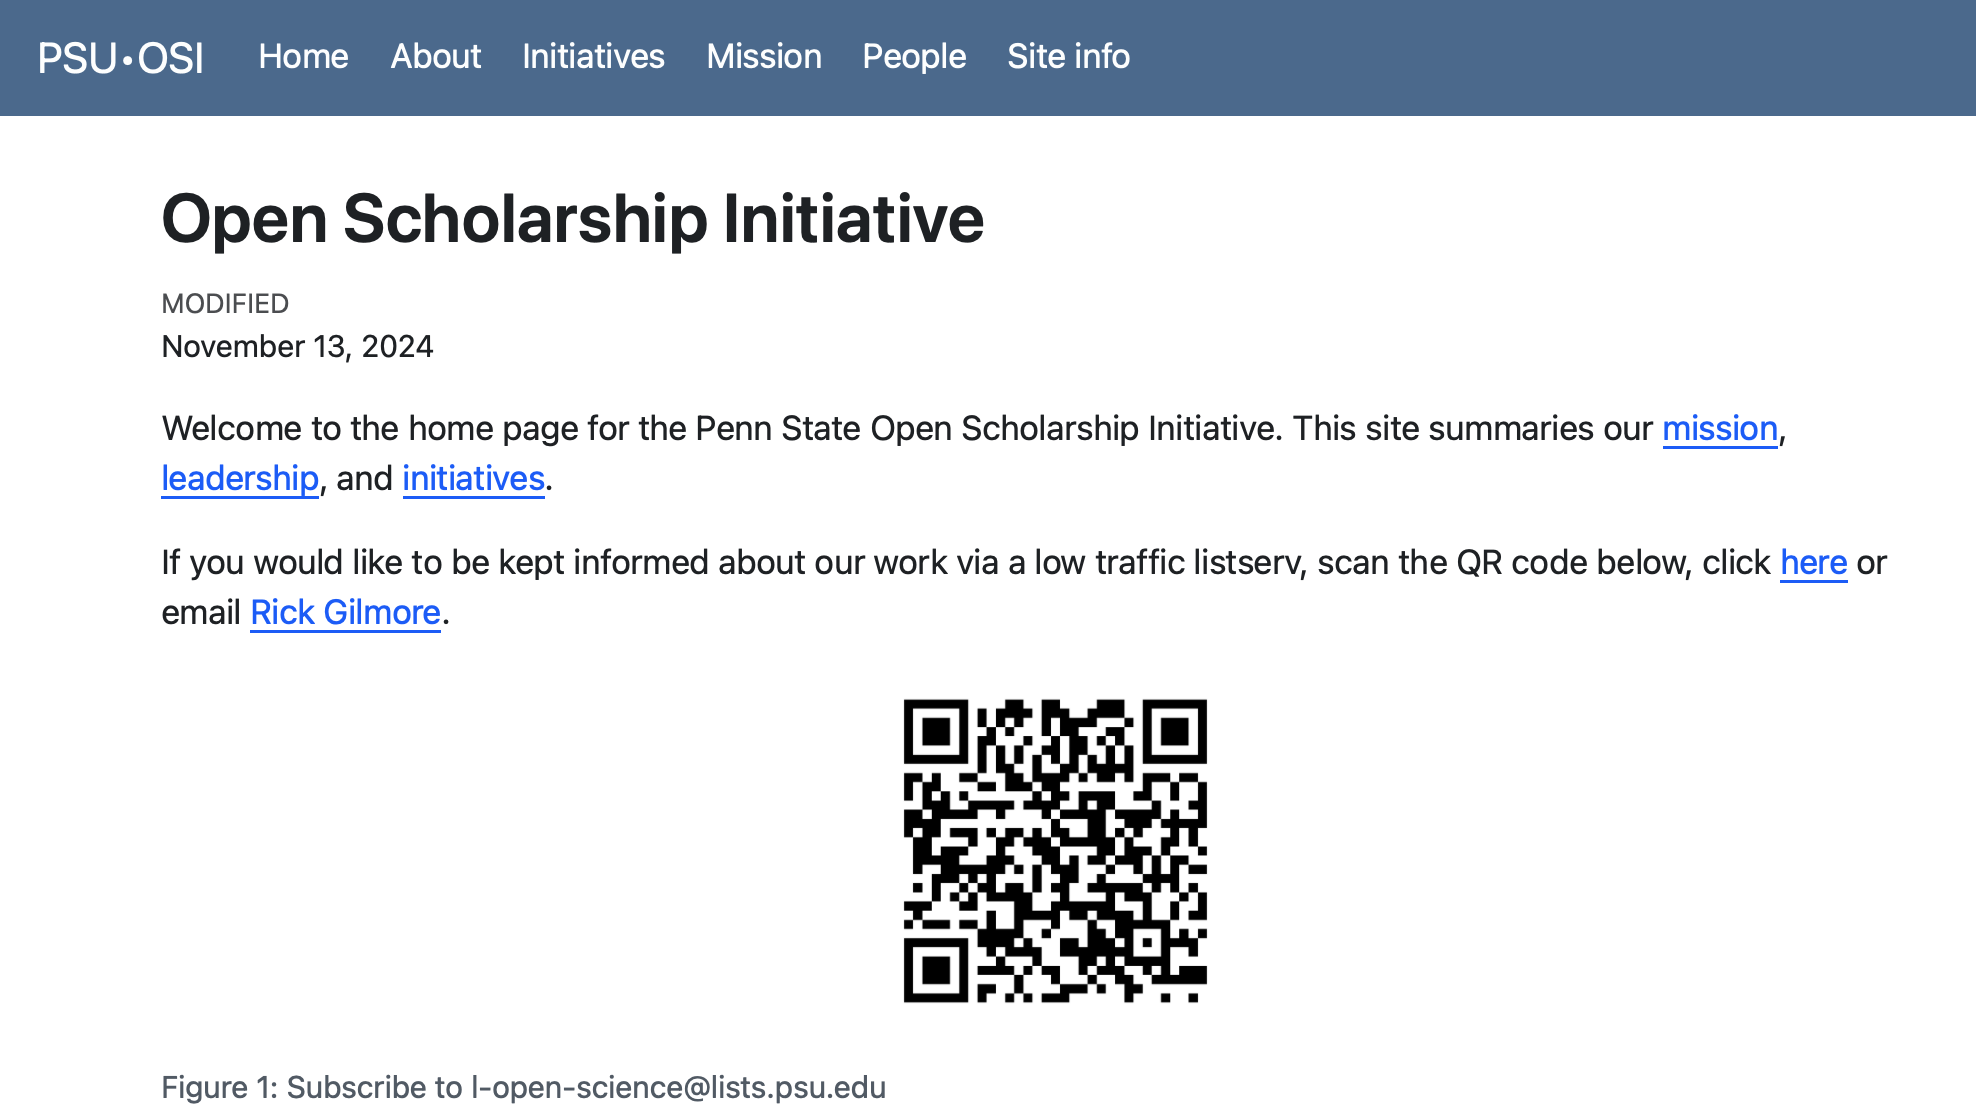
\includegraphics[width=\linewidth,height=1.5625in,keepaspectratio]{img_gilmore_bio/psu-osi.png}
\end{center}

\begin{figure}[H]

{\centering 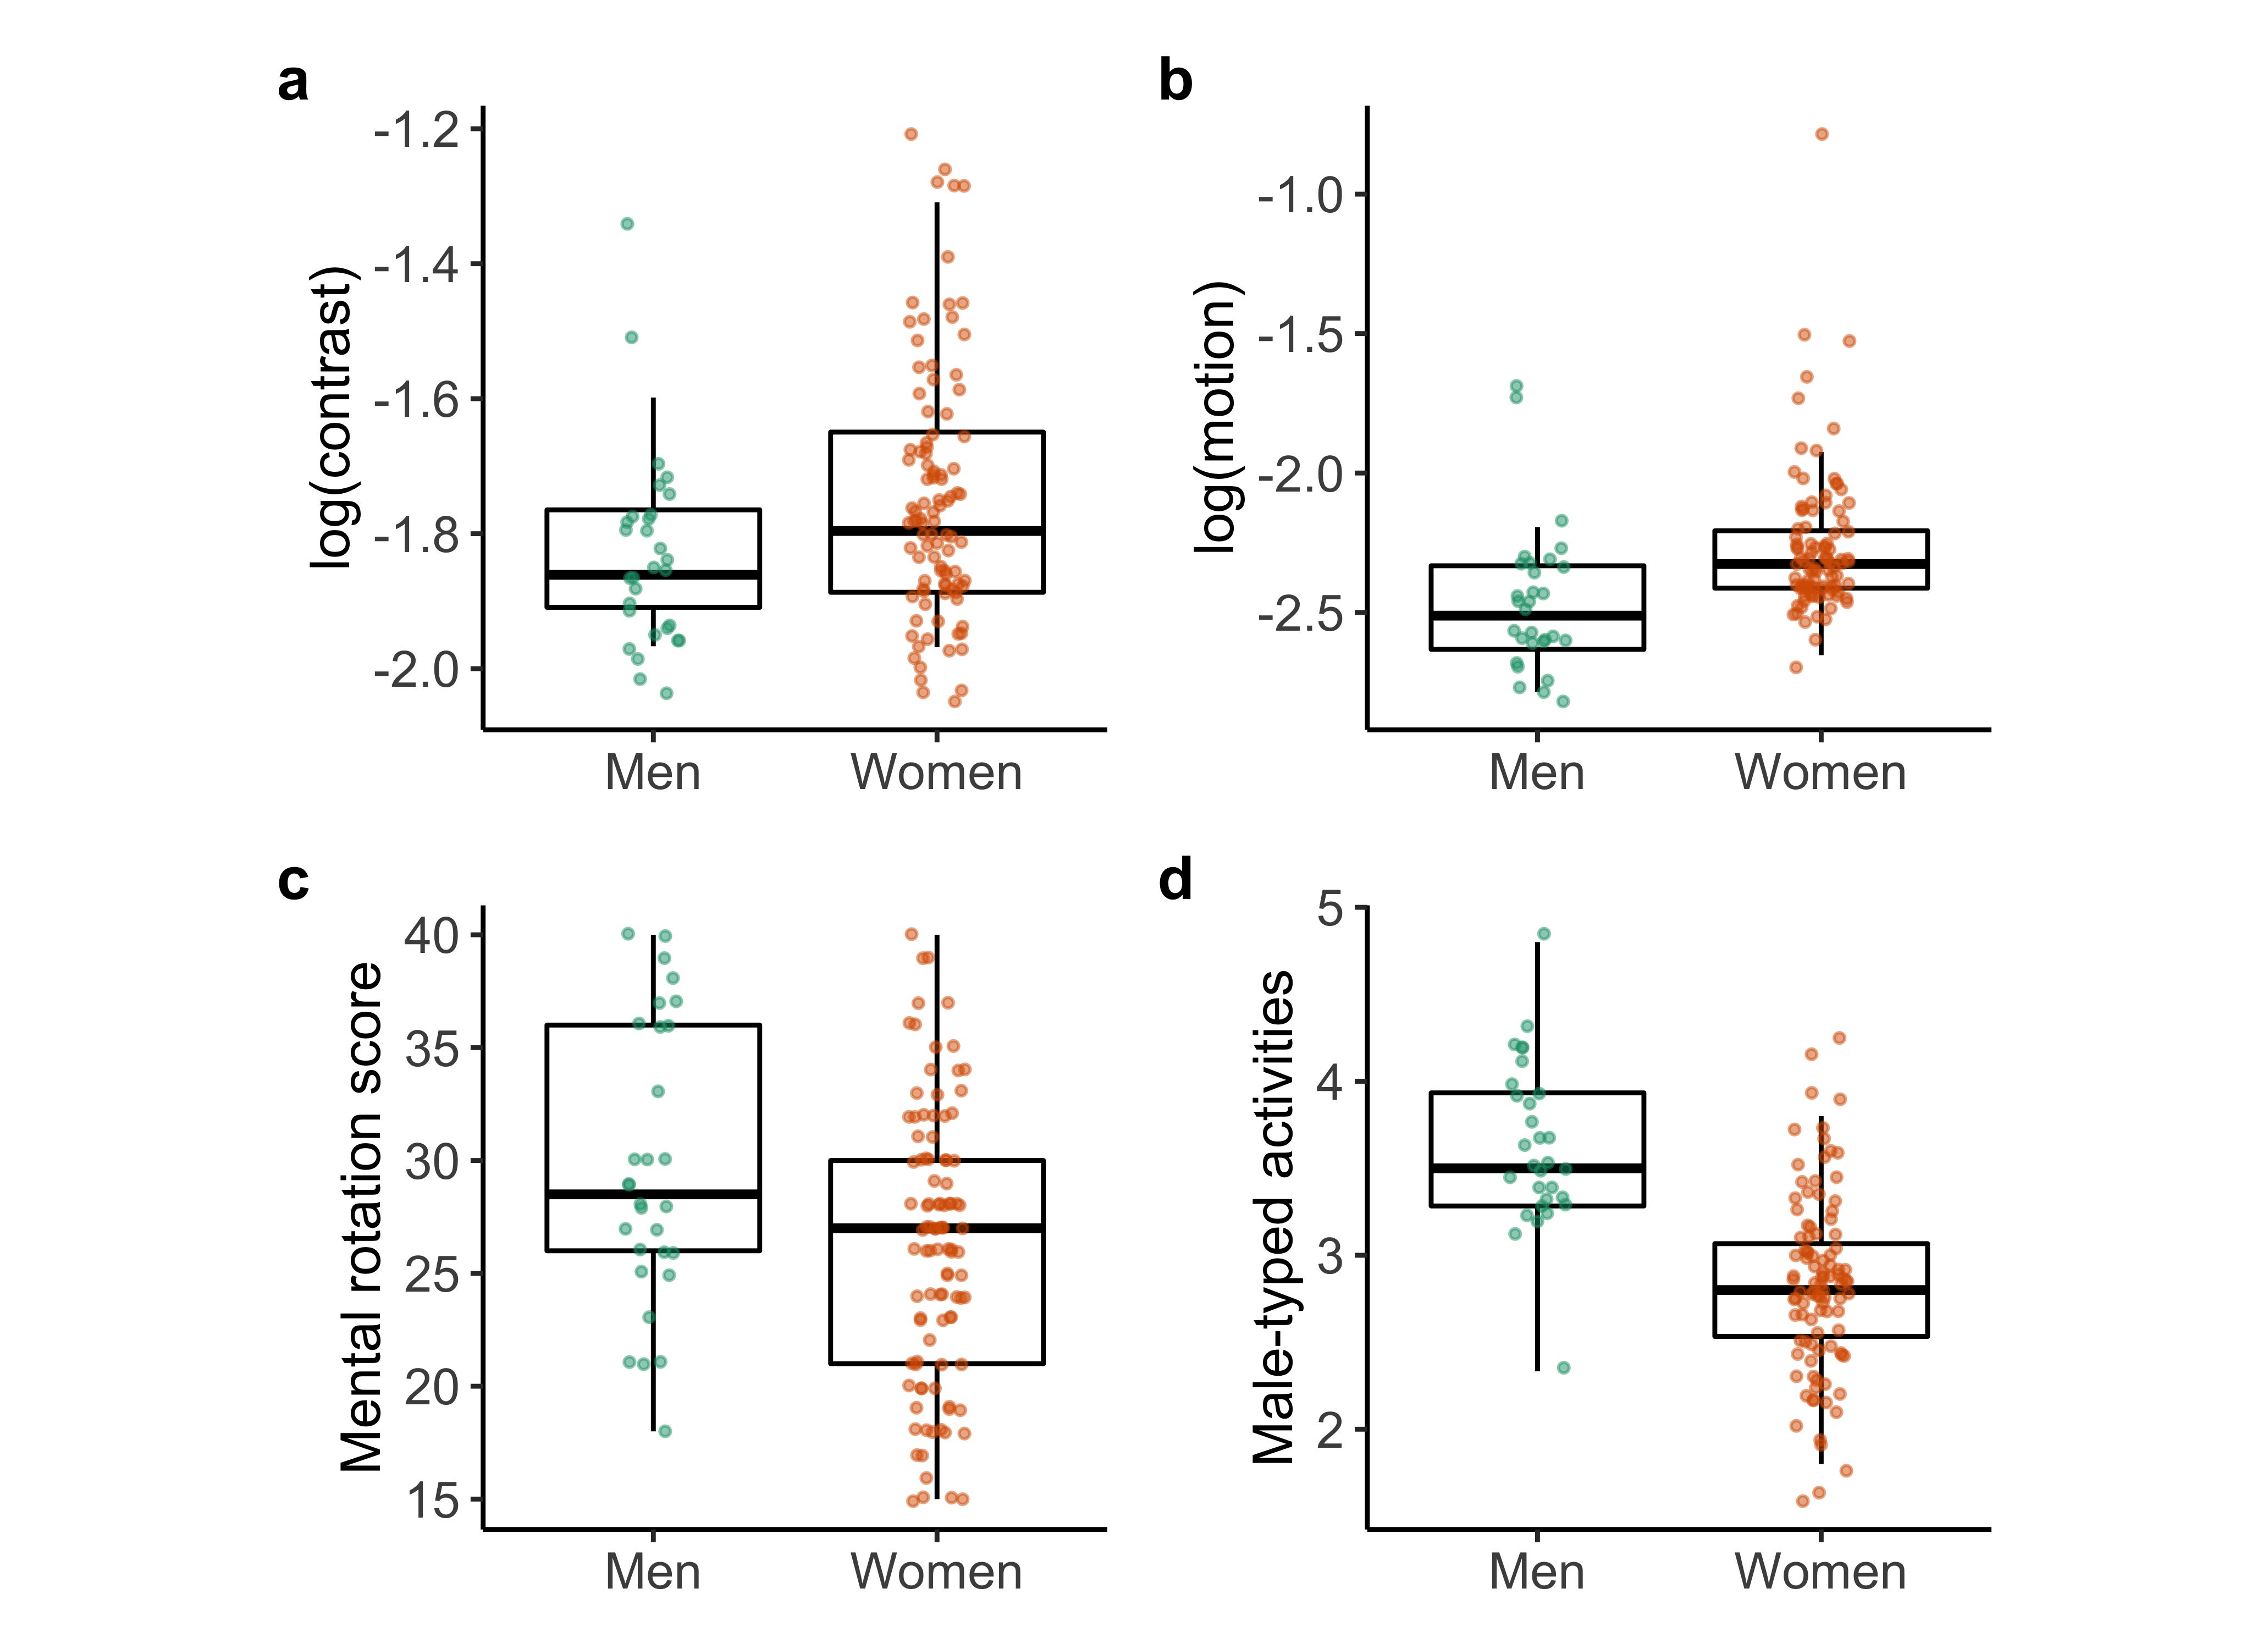
\includegraphics[width=\linewidth,height=2.34375in,keepaspectratio]{img_gilmore_bio/qian-fig-01-boxplots-new.jpg}

}

\caption{Qian, Berenbaum, \& Gilmore (2022)}

\end{figure}%%
\begin{figure}[H]

{\centering 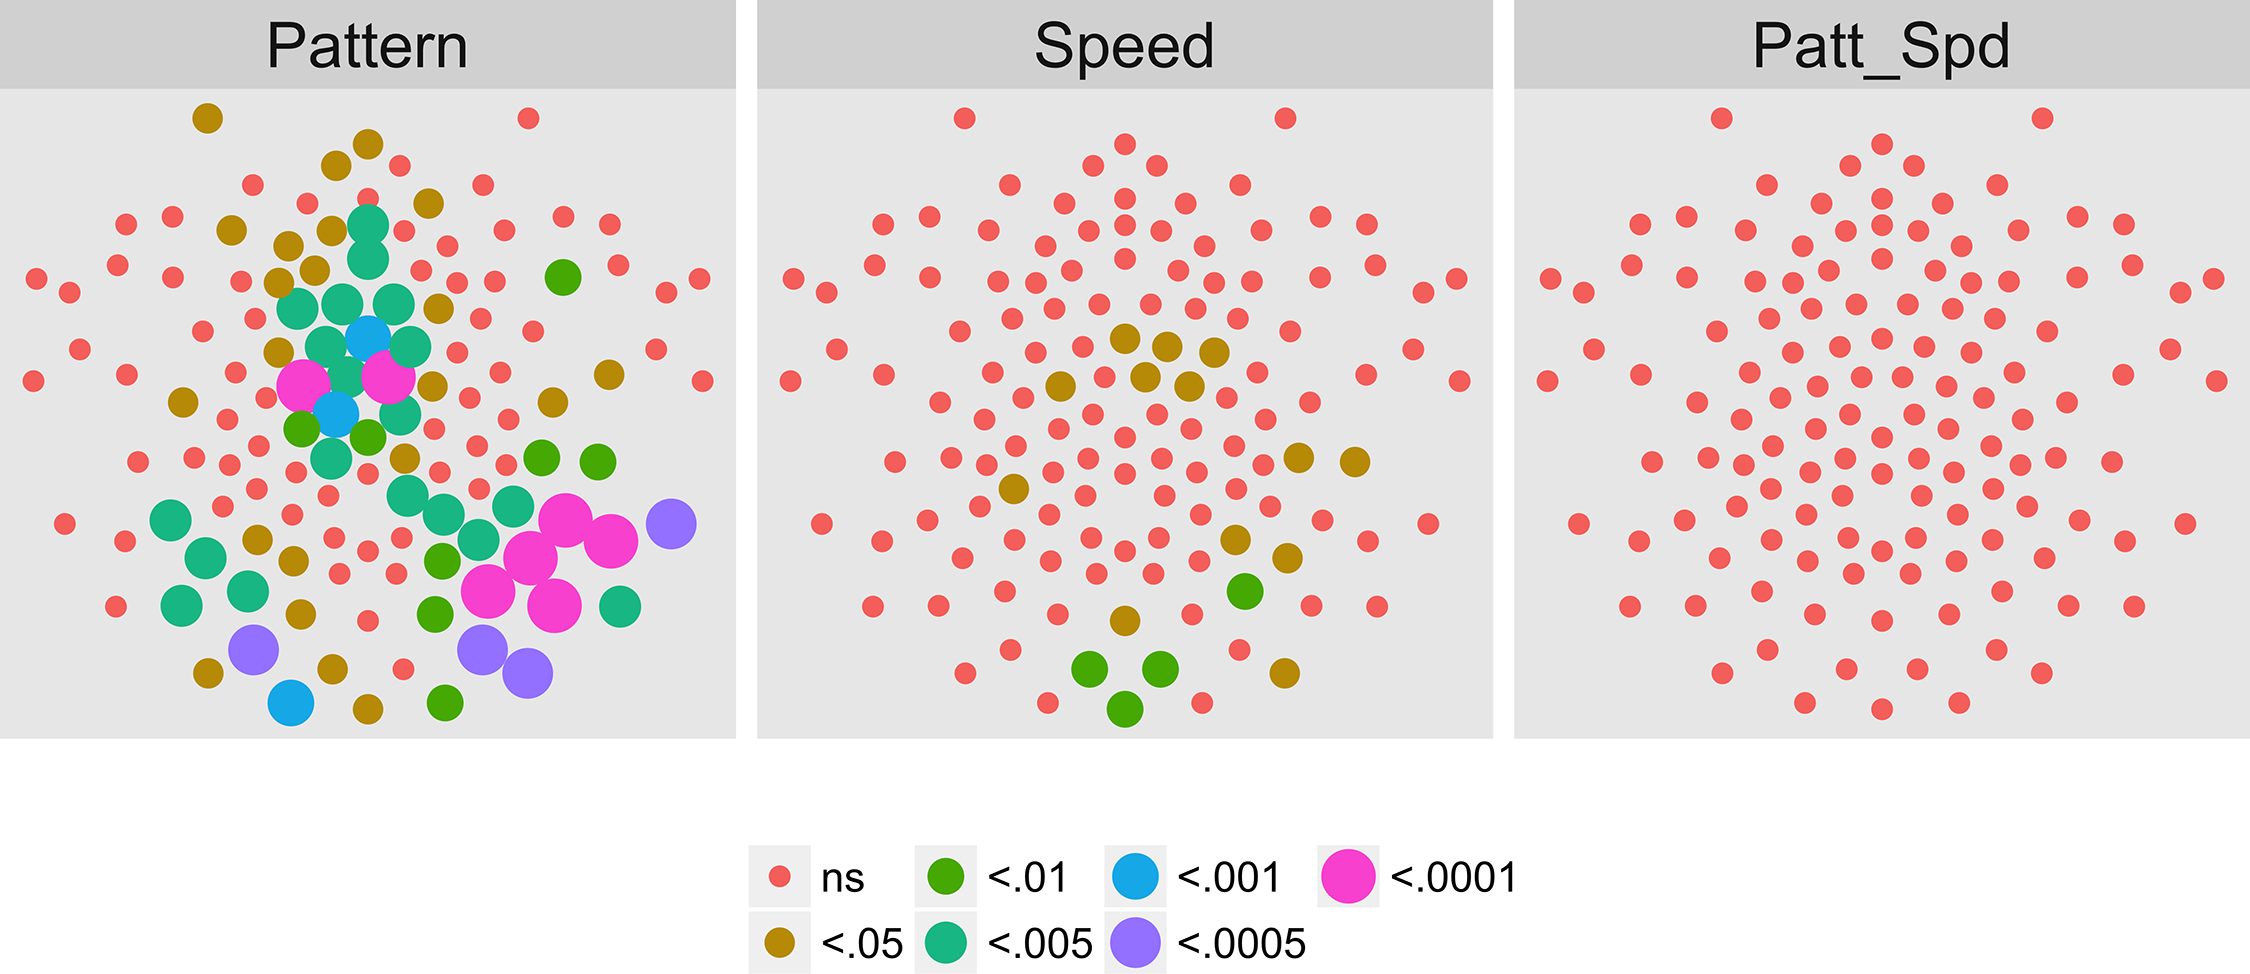
\includegraphics[width=\linewidth,height=2.34375in,keepaspectratio]{img_gilmore_bio/gilmore-thomas-fesi.png}

}

\caption{Gilmore, Thomas, \& Fesi (2016)}

\end{figure}%

\begin{center}\rule{0.5\linewidth}{0.5pt}\end{center}

\begin{figure}[H]

{\centering 
\includegraphics[width=\linewidth,height=1.5625in,keepaspectratio]{wk01-2025-01-16_files/mediabag/Acoustic-Brew-logo.jpg}

}

\caption{https://acousticbrew.org}

\end{figure}%%
\begin{figure}[H]

{\centering 
\includegraphics[width=\linewidth,height=1.5625in,keepaspectratio]{img_gilmore_bio/next-stage-logo.jpg}

}

\caption{https://www.nextstagetheatre.org}

\end{figure}%

\begin{center}
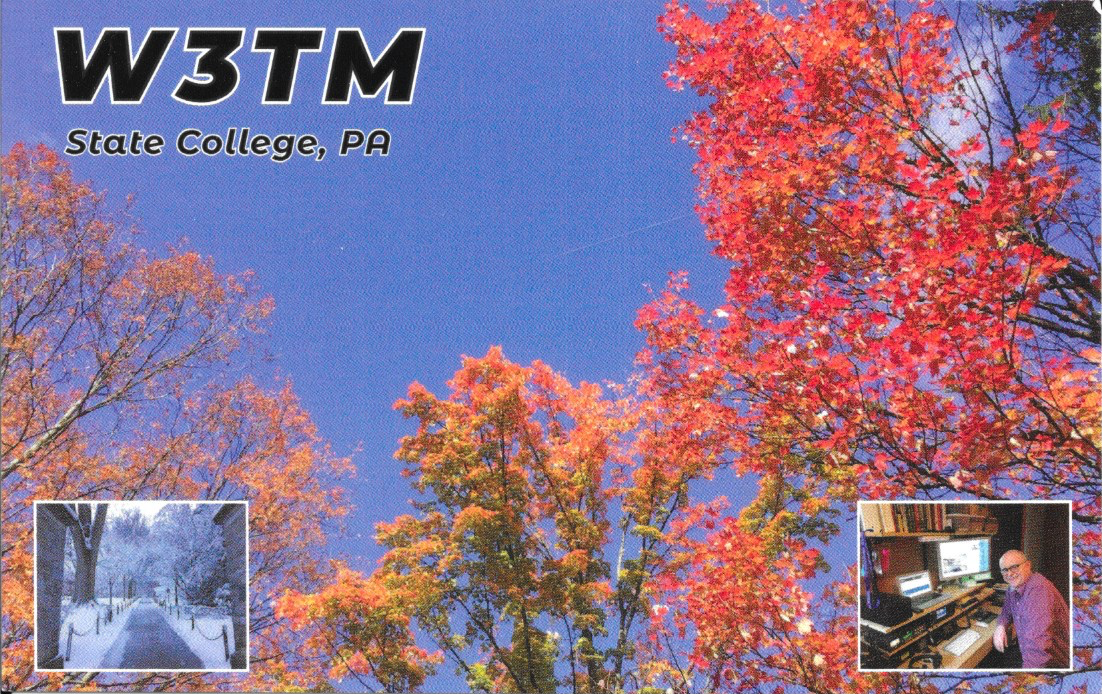
\includegraphics[width=\linewidth,height=1.5625in,keepaspectratio]{wk01-2025-01-16_files/mediabag/w3tm-qsl.png}
\end{center}

\begin{figure}[H]

{\centering 
\includegraphics[width=\linewidth,height=1.5625in,keepaspectratio]{../include/img/cpo-logo.jpg}

}

\caption{https://cpoclub.org}

\end{figure}%

\begin{center}
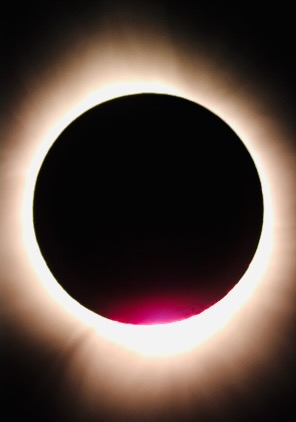
\includegraphics[width=\linewidth,height=1.5625in,keepaspectratio]{../include/img/2024-04-08-151856-Solar-timelapse_thn.jpeg}
\end{center}

\begin{center}
\includegraphics[width=\linewidth,height=1.5625in,keepaspectratio]{../include/img/lola.jpeg}
\end{center}

\subsection{Today's topics}\label{todays-topics}

\begin{itemize}
\tightlist
\item
  Why neuroscience is harder than physics
\item
  Course overview
\item
  Does neuroscience need behavior? Does behavioral science need the
  brain?
\end{itemize}

\section{Why neuroscience is harder than
physics}\label{why-neuroscience-is-harder-than-physics}

\begin{center}\rule{0.5\linewidth}{0.5pt}\end{center}

\pandocbounded{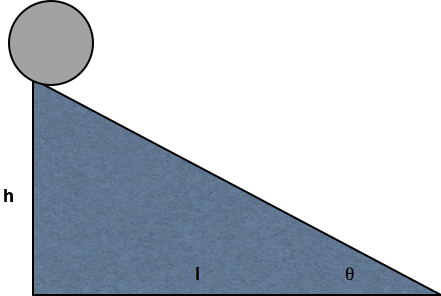
\includegraphics[keepaspectratio]{../include/img/psych-harder-1.jpg}}

\begin{center}\rule{0.5\linewidth}{0.5pt}\end{center}

\pandocbounded{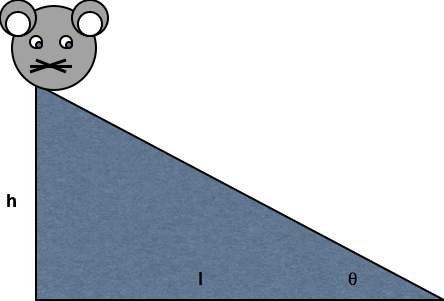
\includegraphics[keepaspectratio]{../include/img/psych-harder-2.jpg}}

\subsection{What do we need to know to answer the
question?}\label{what-do-we-need-to-know-to-answer-the-question}

\begin{itemize}
\tightlist
\item
  What is the state\ldots{}

  \begin{itemize}
  \tightlist
  \item
    Of the world (\(W\))
  \item
    Of the organism

    \begin{itemize}
    \tightlist
    \item
      Body (\(B\))
    \item
      Nervous system (\(N\))
    \item
      Mind (\(M\))
    \end{itemize}
  \end{itemize}
\end{itemize}

\subsection{Nested state spaces}\label{nested-state-spaces}

\begin{figure}[H]

{\centering \pandocbounded{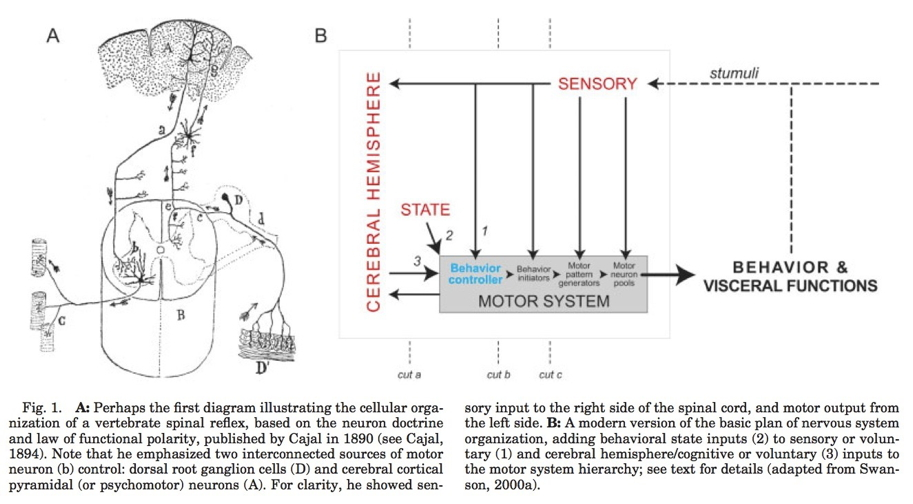
\includegraphics[keepaspectratio]{../include/img/swanson-2005-fig-1.jpg}}

}

\caption{(Swanson, 2005, fig. 1)}

\end{figure}%

\begin{center}\rule{0.5\linewidth}{0.5pt}\end{center}

\pandocbounded{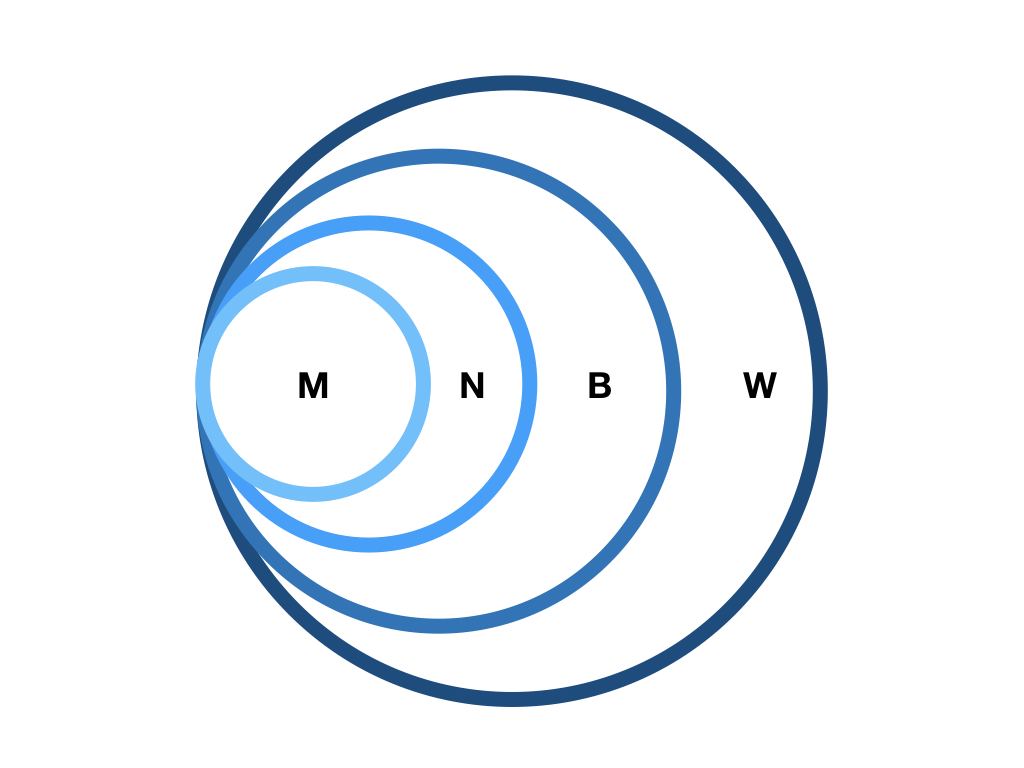
\includegraphics[keepaspectratio]{../include/img/nested-causality-labels.png}}

\subsection{Some states are more easily measured than
others}\label{some-states-are-more-easily-measured-than-others}

\begin{itemize}
\tightlist
\item
  \(W\), \(B\), \(N\) (more or less) \textbf{directly}
\end{itemize}

\begin{center}\rule{0.5\linewidth}{0.5pt}\end{center}

\begin{figure}[H]

{\centering \pandocbounded{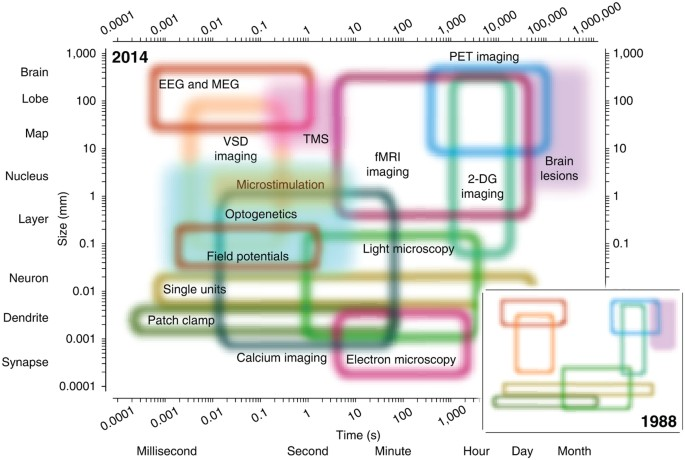
\includegraphics[keepaspectratio]{wk01-2025-01-16_files/mediabag/41593_2014_Article_B.jpg}}

}

\caption{Sejnowski, Churchland, \& Movshon (2014)}

\end{figure}%

\subsection{\texorpdfstring{Mental states
(\(M\))}{Mental states (M)}}\label{mental-states-m}

\begin{itemize}
\tightlist
\item
  Measured \textbf{indirectly}
\item
  Via \(N\), \(B\), \(W\)
\item
  Do you agree?
\end{itemize}

\subsection{\texorpdfstring{What are essential components/dimensions of
\(W\)?}{What are essential components/dimensions of W?}}\label{what-are-essential-componentsdimensions-of-w}

\begin{itemize}
\tightlist
\item
  To explain/understand \(B\) (and \(M\))
\end{itemize}

\subsection{\texorpdfstring{What are essential components/dimensions of
\(B\)?}{What are essential components/dimensions of B?}}\label{what-are-essential-componentsdimensions-of-b}

\begin{itemize}
\tightlist
\item
  To explain/understand
\end{itemize}

\subsection{\texorpdfstring{Brain \& behavior are complex, dynamic
\emph{systems}
with}{Brain \& behavior are complex, dynamic systems with}}\label{brain-behavior-are-complex-dynamic-systems-with}

\begin{itemize}
\tightlist
\item
  Components
\item
  Interactions
\item
  Forces/influences
\item
  Boundaries
\item
  Inputs/outputs/processes
\end{itemize}

\subsection{Systems\ldots{}}\label{systems}

\begin{itemize}
\tightlist
\item
  ``Behave'' or change state across time
\item
  Return to starting state
\item
  Appear to be regulated, controlled, influenced by feedback loops
\item
  \(B(t+1) = f(W(t), B(t), N(t), M(t))\)
\end{itemize}

\subsection{\texorpdfstring{May be analyzed of as
\href{https://en.wikipedia.org/wiki/Network_science}{networks}}{May be analyzed of as networks}}\label{may-be-analyzed-of-as-networks}

\begin{figure}[H]

{\centering \pandocbounded{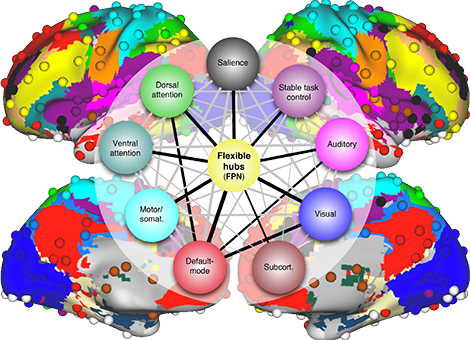
\includegraphics[keepaspectratio]{wk01-2025-01-16_files/mediabag/ColeCoverFlexHub470x.jpg}}

}

\caption{From
https://source.wustl.edu/2013/08/brain-flexible-hub-network-helps-humans-adapt/}

\end{figure}%

\subsection{At multiple levels of
organization\ldots{}}\label{at-multiple-levels-of-organization}

\begin{center}
\pandocbounded{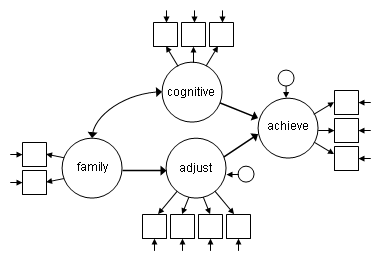
\includegraphics[keepaspectratio]{wk01-2025-01-16_files/mediabag/sem_1.png}}
\end{center}

\begin{center}\rule{0.5\linewidth}{0.5pt}\end{center}

\begin{figure}[H]

{\centering \pandocbounded{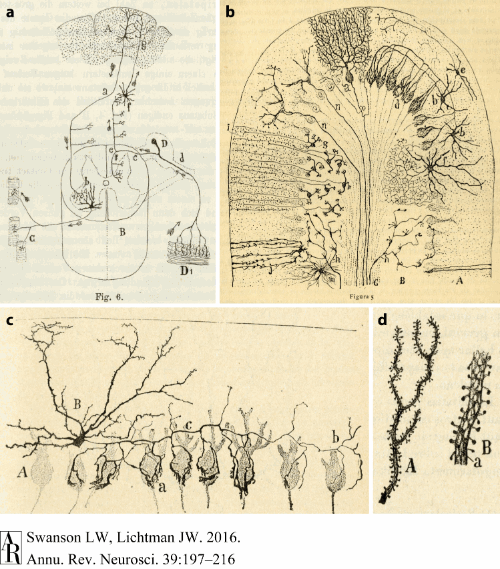
\includegraphics[keepaspectratio]{../include/img/ne390197.f1_thmb.png}}

}

\caption{Swanson \& Lichtman (2016) Figure 1}

\end{figure}%

\begin{center}\rule{0.5\linewidth}{0.5pt}\end{center}

\begin{figure}[H]

{\centering \pandocbounded{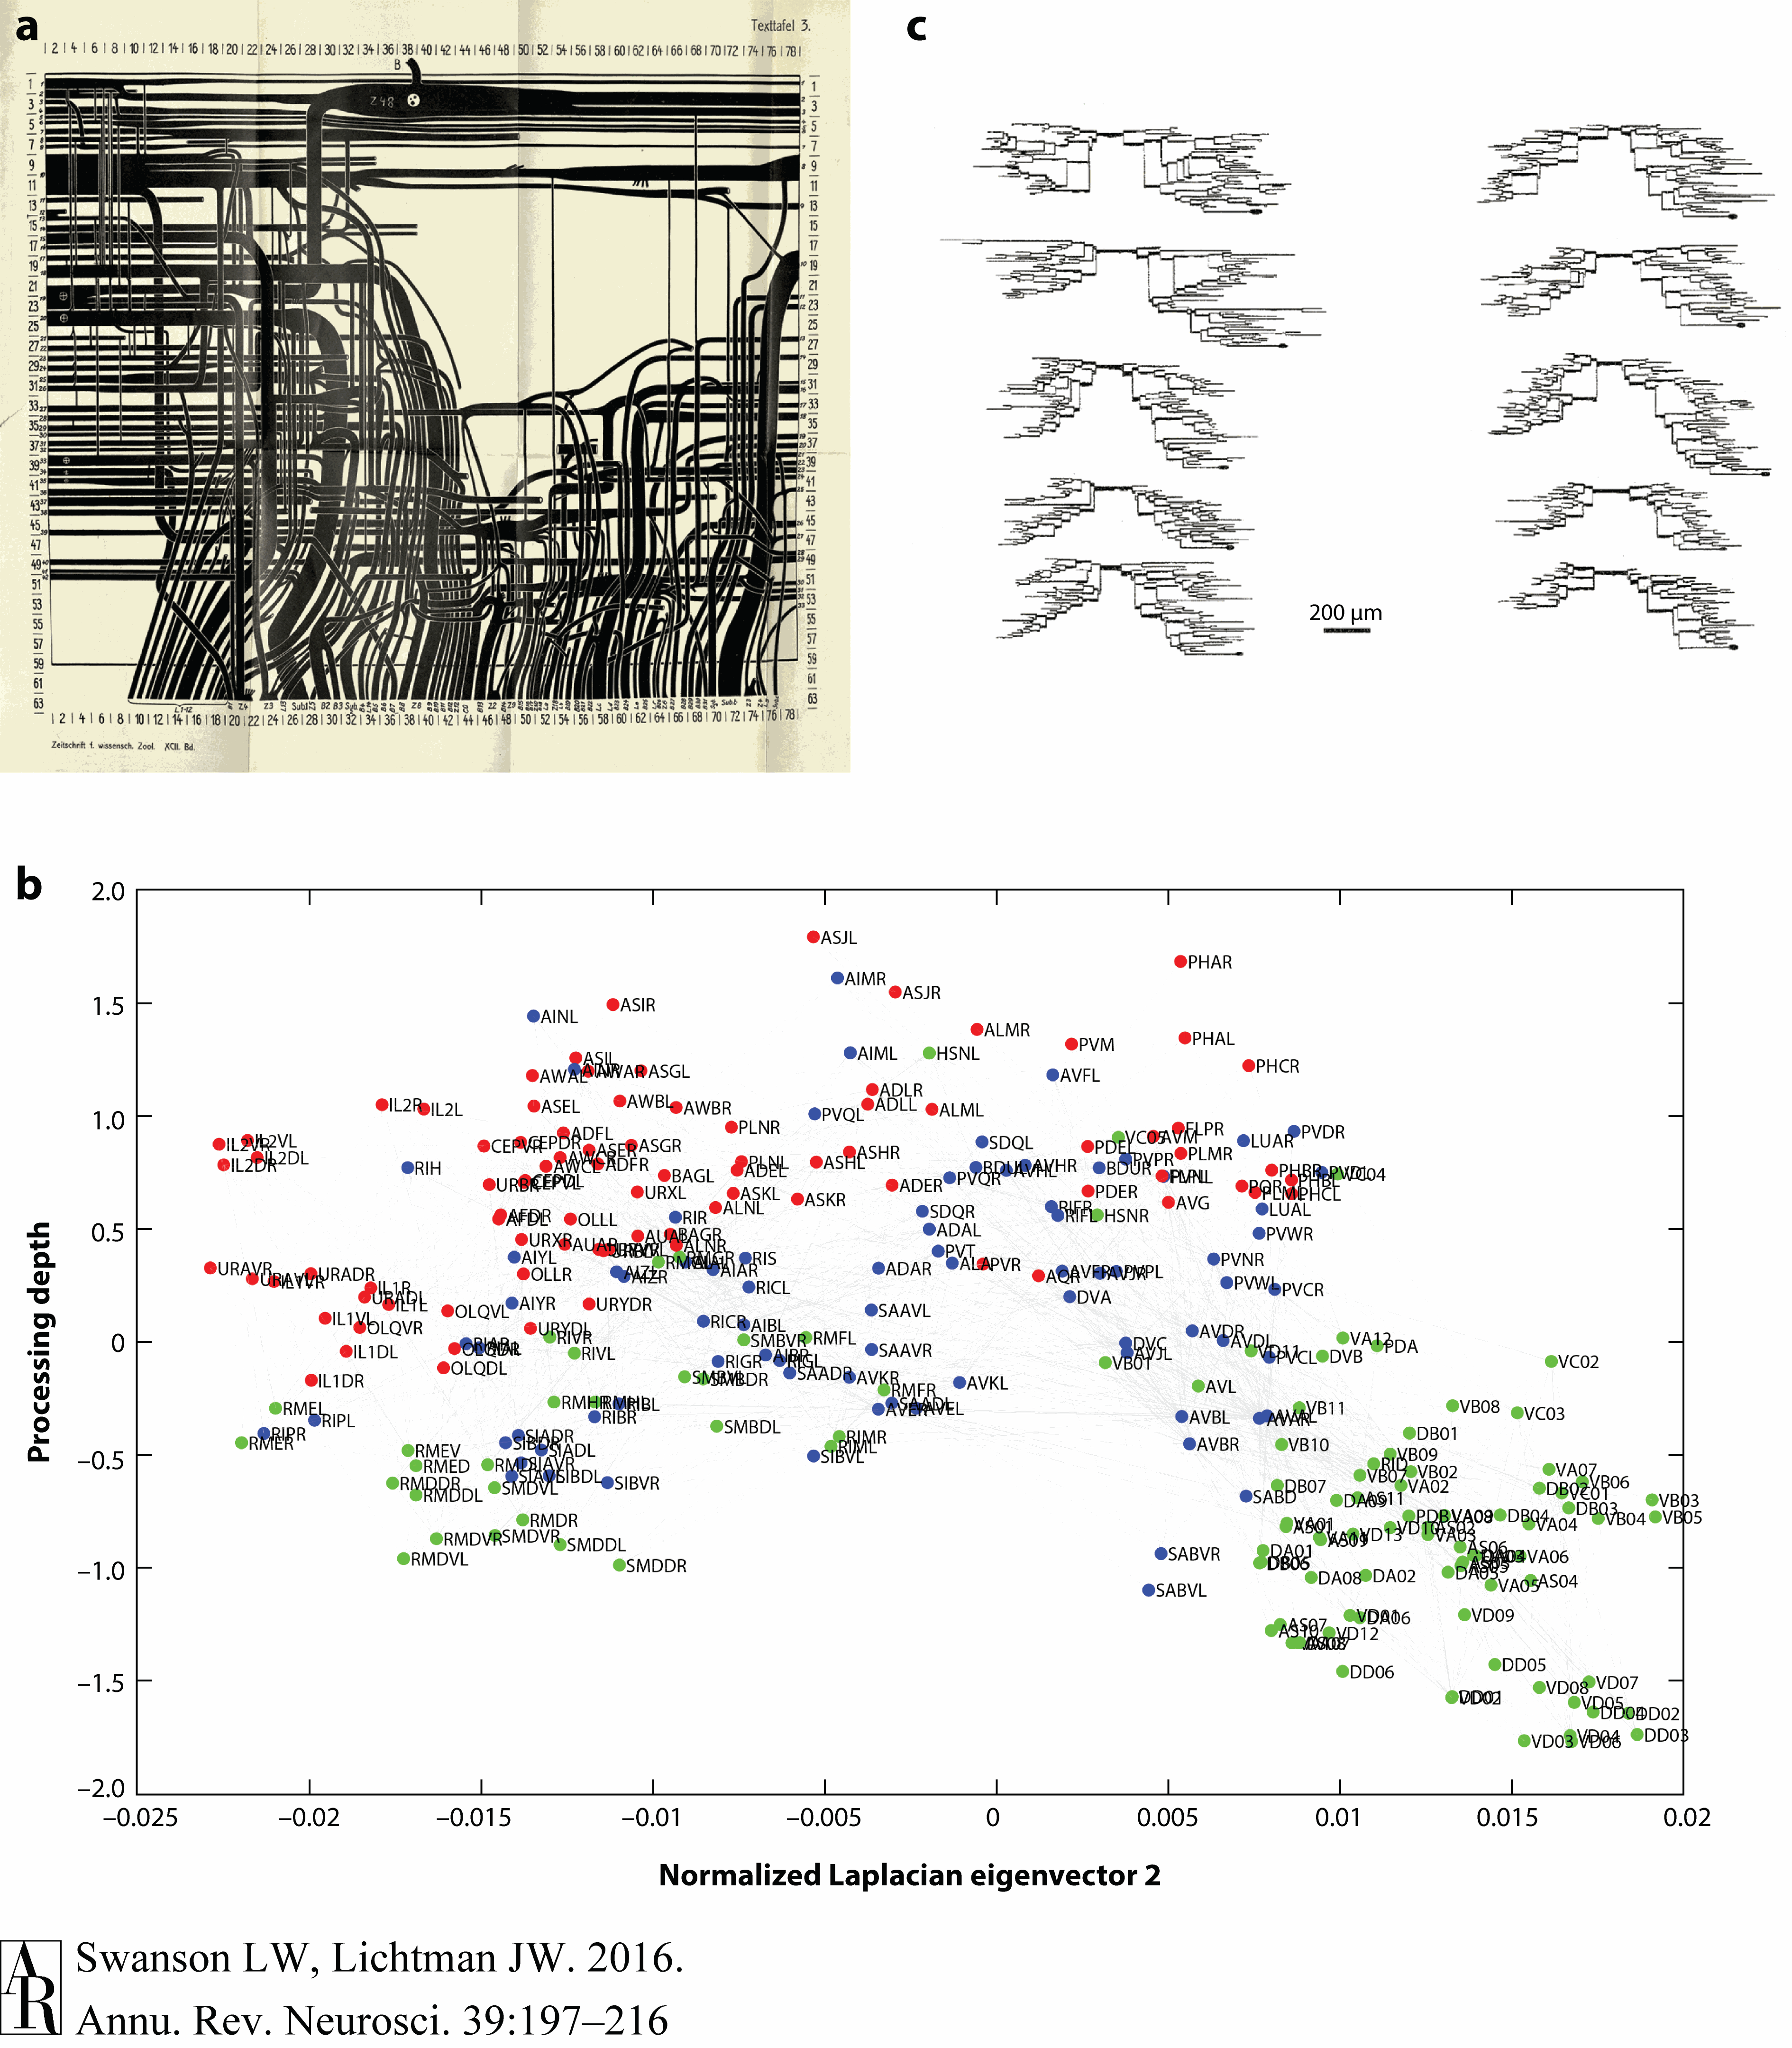
\includegraphics[keepaspectratio]{../include/img/ne390197.f3.png}}

}

\caption{Swanson \& Lichtman (2016) Figure 3}

\end{figure}%

\subsection{Hard to simplify}\label{hard-to-simplify}

\begin{itemize}
\tightlist
\item
  \href{https://en.wikipedia.org/wiki/Spherical_cow}{Consider a
  spherical cow}
\item
  Computation (and memory) often distributed
\item
  Single functions -\textgreater{} multiple parts
\end{itemize}

By Keenan Crane; (The source material is licensed under CC0), CC BY-SA
4.0

\subsection{Single parts -\textgreater{} multiple
functions}\label{single-parts---multiple-functions}

\begin{figure}[H]

{\centering 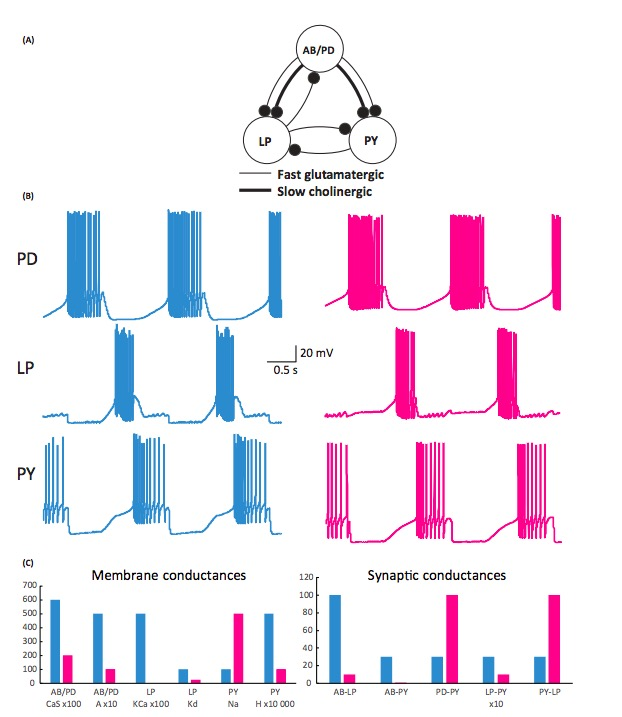
\includegraphics[width=0.6\linewidth,height=\textheight,keepaspectratio]{../include/img/calabrese-2018.jpg}

}

\caption{Calabrese (2018)}

\end{figure}%

\begin{itemize}
\tightlist
\item
  Many circuit wiring patterns
\item
  Similar dynamics
\end{itemize}

\subsection{Biological systems not
``designed''}\label{biological-systems-not-designed}

\begin{itemize}
\tightlist
\item
  \ldots like human-engineered ones
\end{itemize}

\begin{figure}[H]

{\centering \pandocbounded{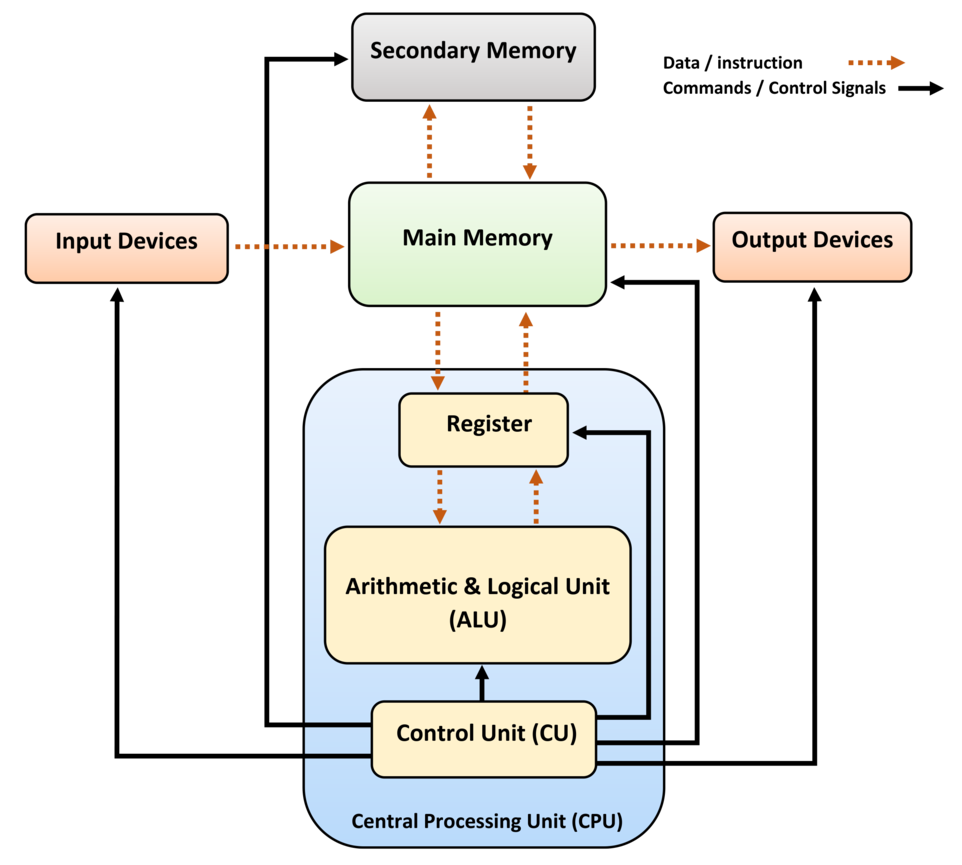
\includegraphics[keepaspectratio]{../include/img/Computer_architecture_block_diagram.png}}

}

\caption{https://en.wikipedia.org/wiki/Computer\_architecture}

\end{figure}%

\subsection{Studying such systems is hard
because\ldots{}}\label{studying-such-systems-is-hard-because}

\begin{itemize}
\tightlist
\item
  Change structure/function over time
\item
  Hard to measure what is being exchanged, what is being
  \emph{controlled}
\end{itemize}

\begin{center}\rule{0.5\linewidth}{0.5pt}\end{center}

\begin{figure}[H]

{\centering \pandocbounded{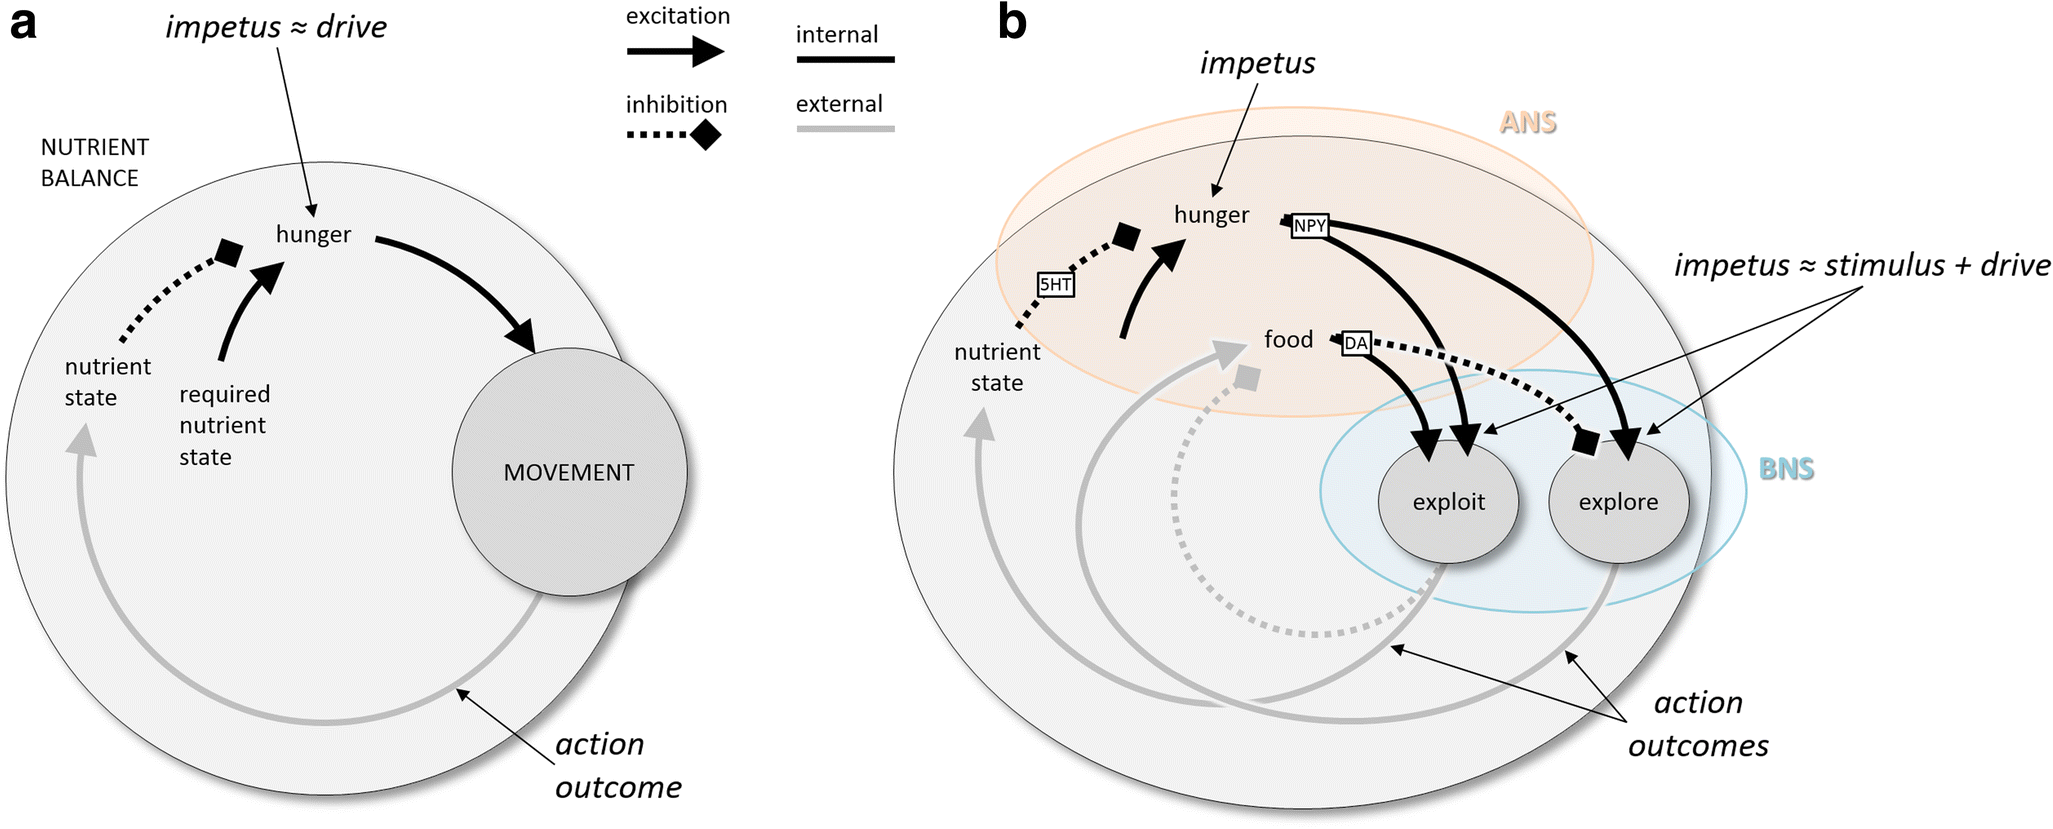
\includegraphics[keepaspectratio]{wk01-2025-01-16_files/mediabag/13414_2019_1760_Fig3.png}}

}

\caption{(Cisek, 2019, fig. 3). Schematic behavioral control systems.
(A) When the current nutrient state deviates from a desired state,
locomotion is initiated, ultimately bringing the animal to a more
desirable state. (B) Elaboration of nutrient state control into a
high-level controller (ANS) and a lower-level controller (BNS) capable
of two modes of locomotion, local exploitation, and long-range
exploration. 5HT, serotonin; ANS/BNS, apical/blastoporal nervous system;
DA, dopamine; NPY, neuropeptide Y}

\end{figure}%

\subsection{Assumptions are
problematic}\label{assumptions-are-problematic}

\begin{figure}[H]

{\centering \pandocbounded{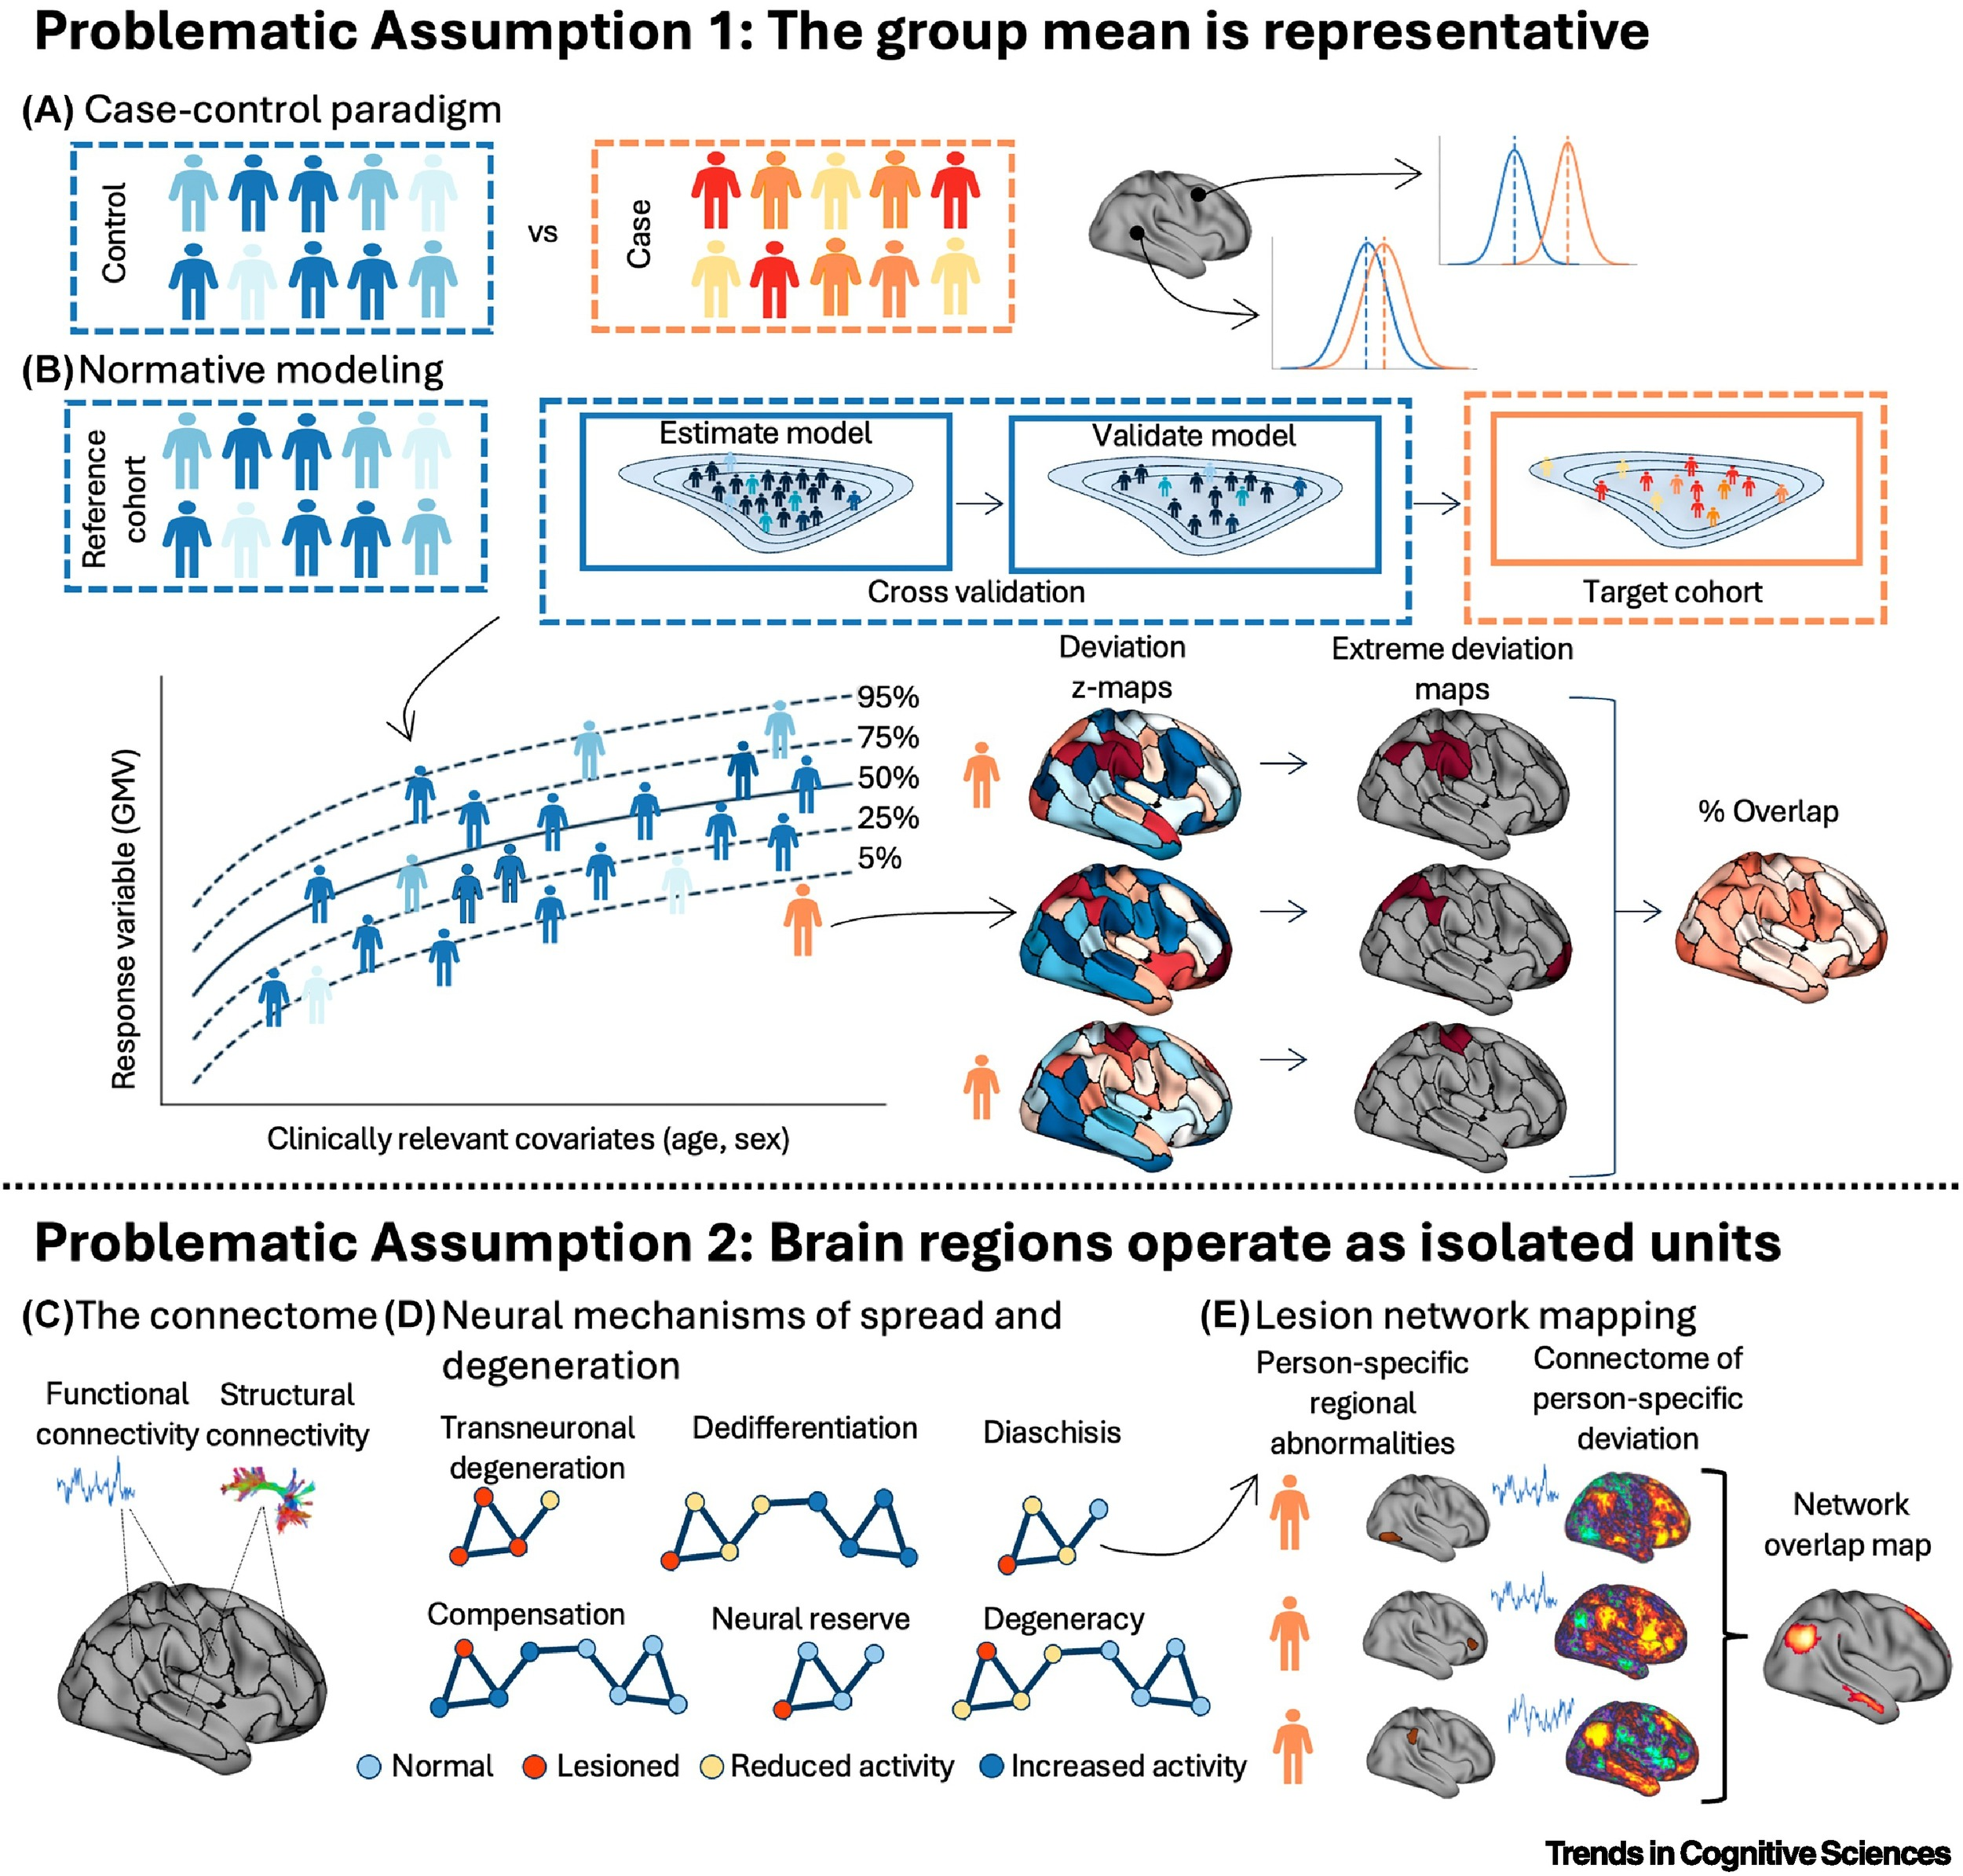
\includegraphics[keepaspectratio]{../include/img/segal-2024-fig-01.jpg}}

}

\caption{Segal et al. (2024)}

\end{figure}%

\section{Course overview}\label{course-overview}

\subsection{Goals}\label{goals}

\begin{itemize}
\tightlist
\item
  Master fundamentals of neuroscientific concepts and facts
\item
  Prepare to read primary source literature in social, behavioral,
  cognitive, affective, and clinical neuroscience
\end{itemize}

\subsection{Structure}\label{structure}

\url{https://psu-psychology.github.io/psy-511-scan-fdns-2025-spring/}

\subsection{Questions}\label{questions}

\begin{itemize}
\tightlist
\item
  What is the basic organizational plan of the nervous system?
\item
  How do neurons work?
\item
  How do neurons connected in networks achieve behavioral goals?
\item
  How does the nervous system develop? How has it evolved?
\item
  How do disorders of the mind reveal themselves in the nervous system?
\end{itemize}

\subsection{Approach}\label{approach}

\begin{itemize}
\tightlist
\item
  Brain architecture (neuroanatomy)
\item
  Brain function (neurophysiology)
\item
  Brain communication (neurochemistry)
\item
  Changes over evolutionary and developmental time
\end{itemize}

\subsection{Approach}\label{approach-1}

\begin{itemize}
\tightlist
\item
  The nervous system as an information processing system
\end{itemize}

\begin{figure}[H]

{\centering \pandocbounded{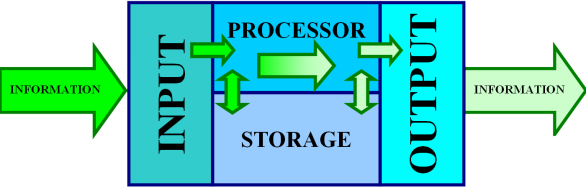
\includegraphics[keepaspectratio]{../include/img/Information_processing_system.PNG}}

}

\caption{Wikipedia}

\end{figure}%

\subsection{Mindful of limitations in brain/computer
metaphors}\label{mindful-of-limitations-in-braincomputer-metaphors}

\begin{figure}[H]

{\centering \pandocbounded{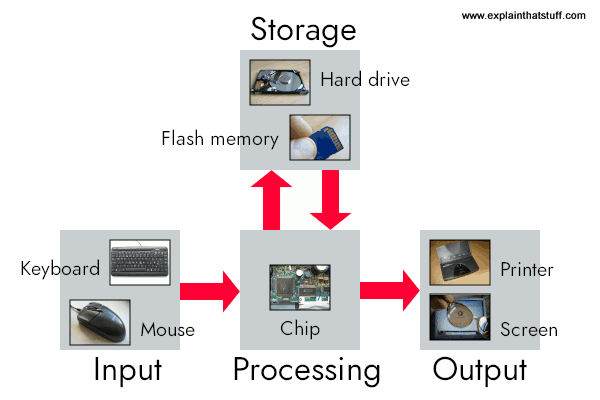
\includegraphics[keepaspectratio]{wk01-2025-01-16_files/mediabag/how-computer-works.png}}

}

\caption{https://www.explainthatstuff.com/howcomputerswork.html}

\end{figure}%

\subsection{Or inspired by richer
metaphors}\label{or-inspired-by-richer-metaphors}

\begin{figure}[H]

{\centering \pandocbounded{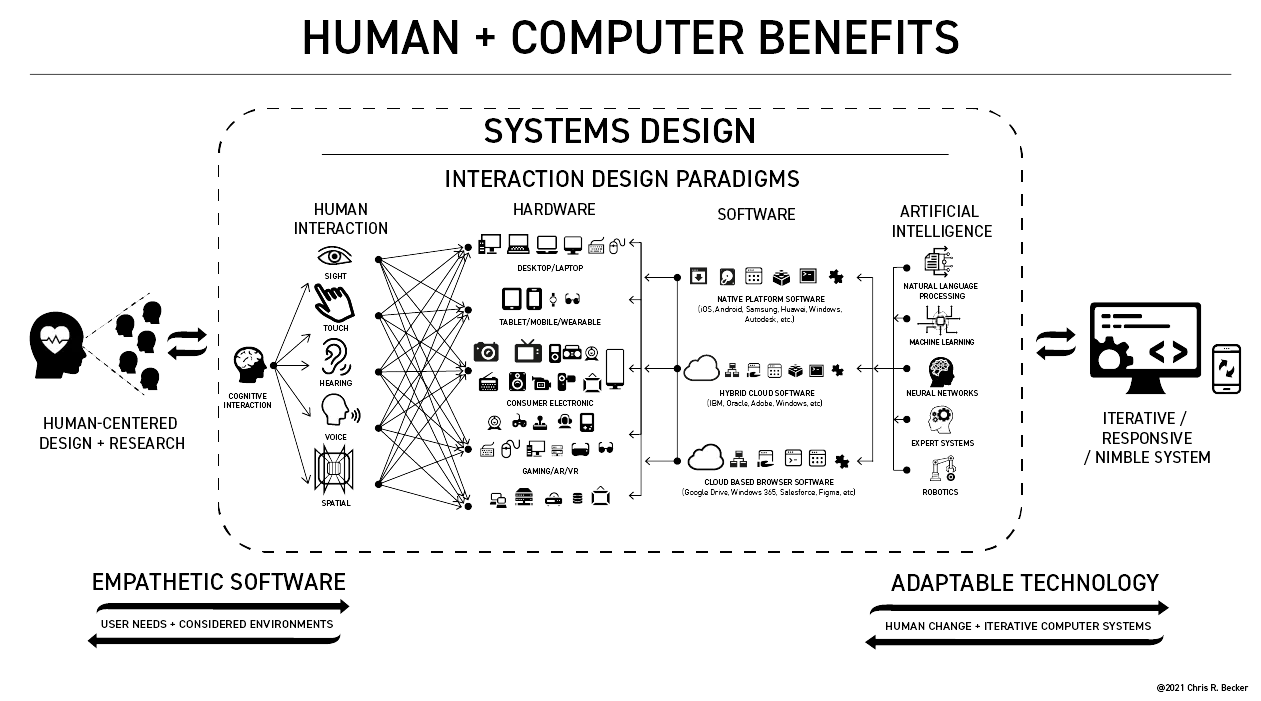
\includegraphics[keepaspectratio]{../include/img/1*QvKZpHrmz1nWyK4VfY2VTg.png}}

}

\caption{Becker (2021)}

\end{figure}%

\subsection{Inputs}\label{inputs}

\begin{itemize}
\tightlist
\item
  From environment, body, brain
\end{itemize}

\subsection{Processing}\label{processing}

\begin{itemize}
\tightlist
\item
  Current inputs + brain state + body state + possible future
  states\ldots{}
\item
  Stored information
\item
  Physiological \& behavioral goals
\end{itemize}

\begin{center}\rule{0.5\linewidth}{0.5pt}\end{center}

\begin{figure}[H]

{\centering \pandocbounded{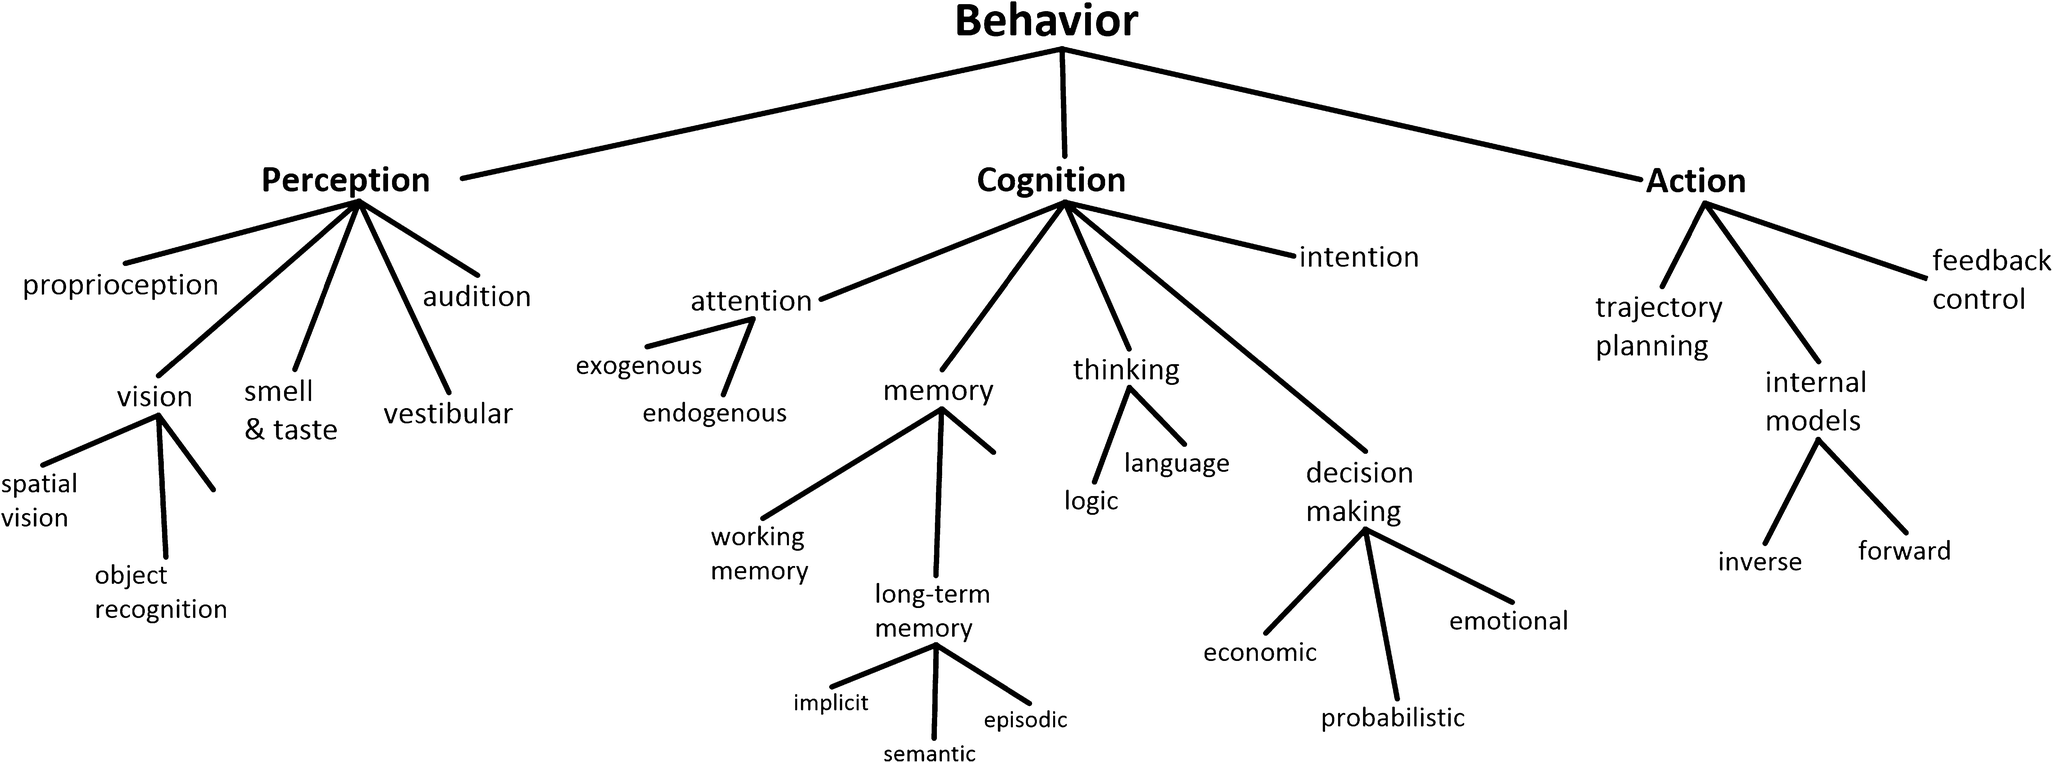
\includegraphics[keepaspectratio]{wk01-2025-01-16_files/mediabag/13414_2019_1760_Fig1.png}}

}

\caption{(Cisek, 2019, fig. 1)}

\end{figure}%

\begin{center}\rule{0.5\linewidth}{0.5pt}\end{center}

\subsection{Outputs}\label{outputs}

\begin{itemize}
\tightlist
\item
  To brain, body, environment
\end{itemize}

\subsection{Mapping structures to
functions\ldots{}}\label{mapping-structures-to-functions}

\begin{figure}[H]

{\centering \pandocbounded{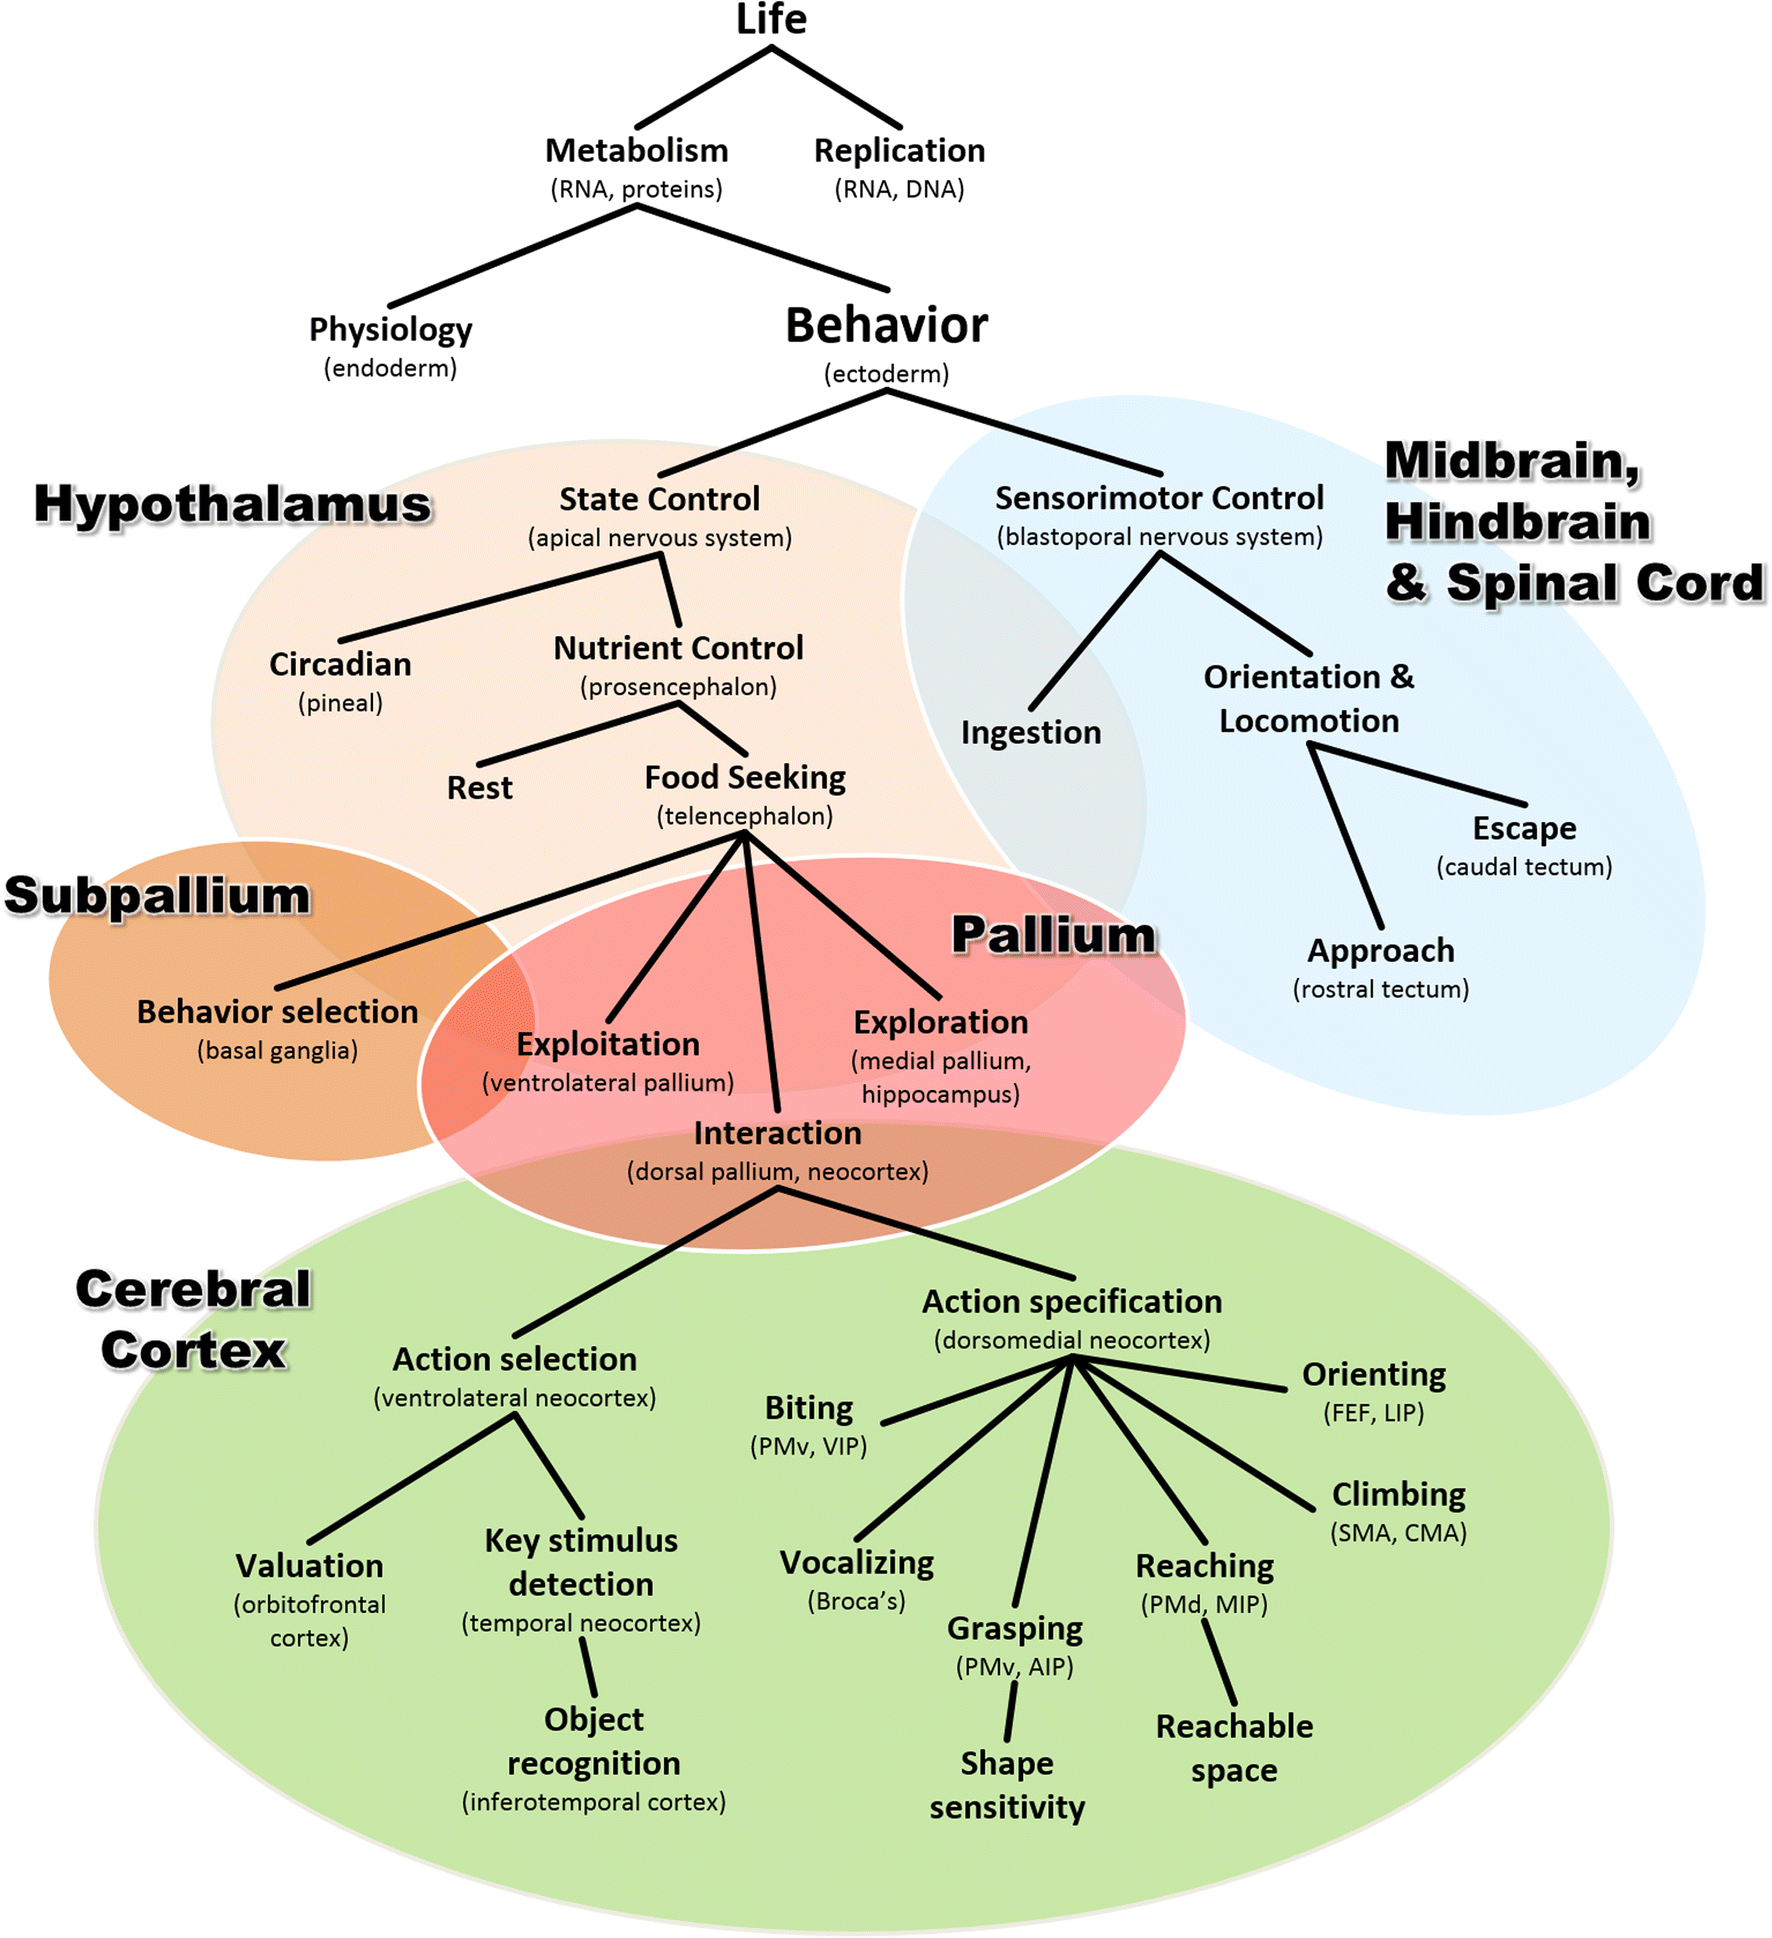
\includegraphics[keepaspectratio]{wk01-2025-01-16_files/mediabag/13414_2019_1760_Fig8.png}}

}

\caption{Cisek (2019) Figure 8}

\end{figure}%

\subsection{\texorpdfstring{And \emph{vice
versa}?}{And vice versa?}}\label{and-vice-versa}

\begin{figure}[H]

{\centering \pandocbounded{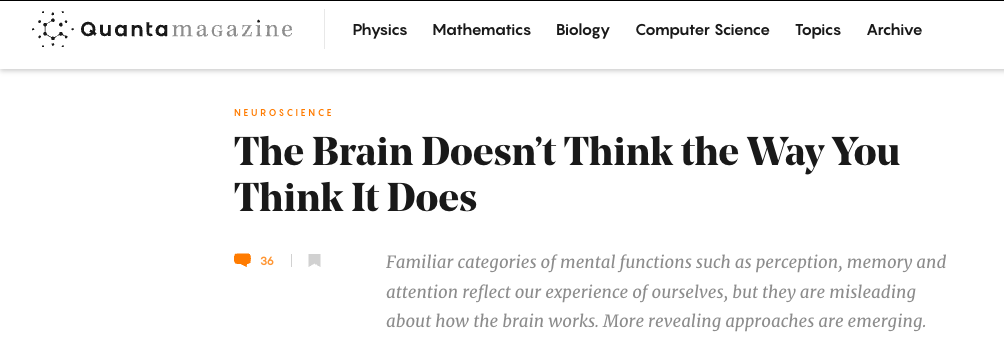
\includegraphics[keepaspectratio]{../include/img/quanta-2021.png}}

}

\caption{Cepelewicz (2021)}

\end{figure}%

\begin{center}\rule{0.5\linewidth}{0.5pt}\end{center}

\begin{quote}
``The brainwide representation of behavioral variables suggests that
information encoded nearly anywhere in the forebrain is combined with
behavioral state variables into a mixed representation\ldots Our data
indicate that it happens as early as primary sensory cortex.''
\end{quote}

Stringer et al. (2019)

\subsection{And do we have the right ``psychological''
structures?}\label{and-do-we-have-the-right-psychological-structures}

\begin{quote}
Psychological sciences have identified a wealth of cognitive processes
and behavioral phenomena, yet struggle to produce cumulative knowledge.
Progress is hamstrung by siloed scientific traditions and a focus on
explanation over prediction\ldots{}
\end{quote}

Eisenberg et al. (2019)

\begin{center}\rule{0.5\linewidth}{0.5pt}\end{center}

\begin{quote}
\ldots two issues that are particularly damaging for the study of
\textbf{multifaceted constructs like self-regulation}\ldots We conclude
that self-regulation lacks coherence as a construct\ldots{}
\end{quote}

Eisenberg et al. (2019)

\subsection{``Behavioural biologists don't agree on what constitutes
behaviour''}\label{behavioural-biologists-dont-agree-on-what-constitutes-behaviour}

\begin{quote}
Behavioural biology is a major discipline within biology, centred on the
key concept of `behaviour'. But how is `behaviour' defined, and how
should it be defined? We outline what characteristics we believe a
scientific definition should have, and why we think it is
important\ldots{}
\end{quote}

Levitis, Lidicker, \& Freund (2009)

\begin{center}\rule{0.5\linewidth}{0.5pt}\end{center}

\begin{quote}
\ldots that a definition have these traits. We then examine the range of
available published definitions for behaviour.
\end{quote}

Levitis et al. (2009)

\begin{center}\rule{0.5\linewidth}{0.5pt}\end{center}

\begin{quote}
Finding no consensus, we present survey responses from 174 members of
three behaviour-focused scientific societies as to their understanding
of the term. Here again, we find surprisingly widespread disagreement as
to what qualifies as behaviour. Respondents contradict
themselves\ldots{}
\end{quote}

Levitis et al. (2009)

\begin{center}\rule{0.5\linewidth}{0.5pt}\end{center}

\begin{quote}
\ldots each other, and published definitions, indicating that they are
using individually variable intuitive, rather than codified, meanings of
`behaviour.'
\end{quote}

Levitis et al. (2009)

\begin{center}\rule{0.5\linewidth}{0.5pt}\end{center}

\begin{quote}
We offer a new definition, based largely on survey responses:
``Behaviour is the internally coordinated responses (actions or
inactions) of whole living organisms (individuals or groups) to internal
and/or external stimuli, excluding responses more easily understood as
developmental changes.''
\end{quote}

Levitis et al. (2009)

\subsection{Sciences of complexity}\label{sciences-of-complexity}

\begin{figure}[H]

{\centering \pandocbounded{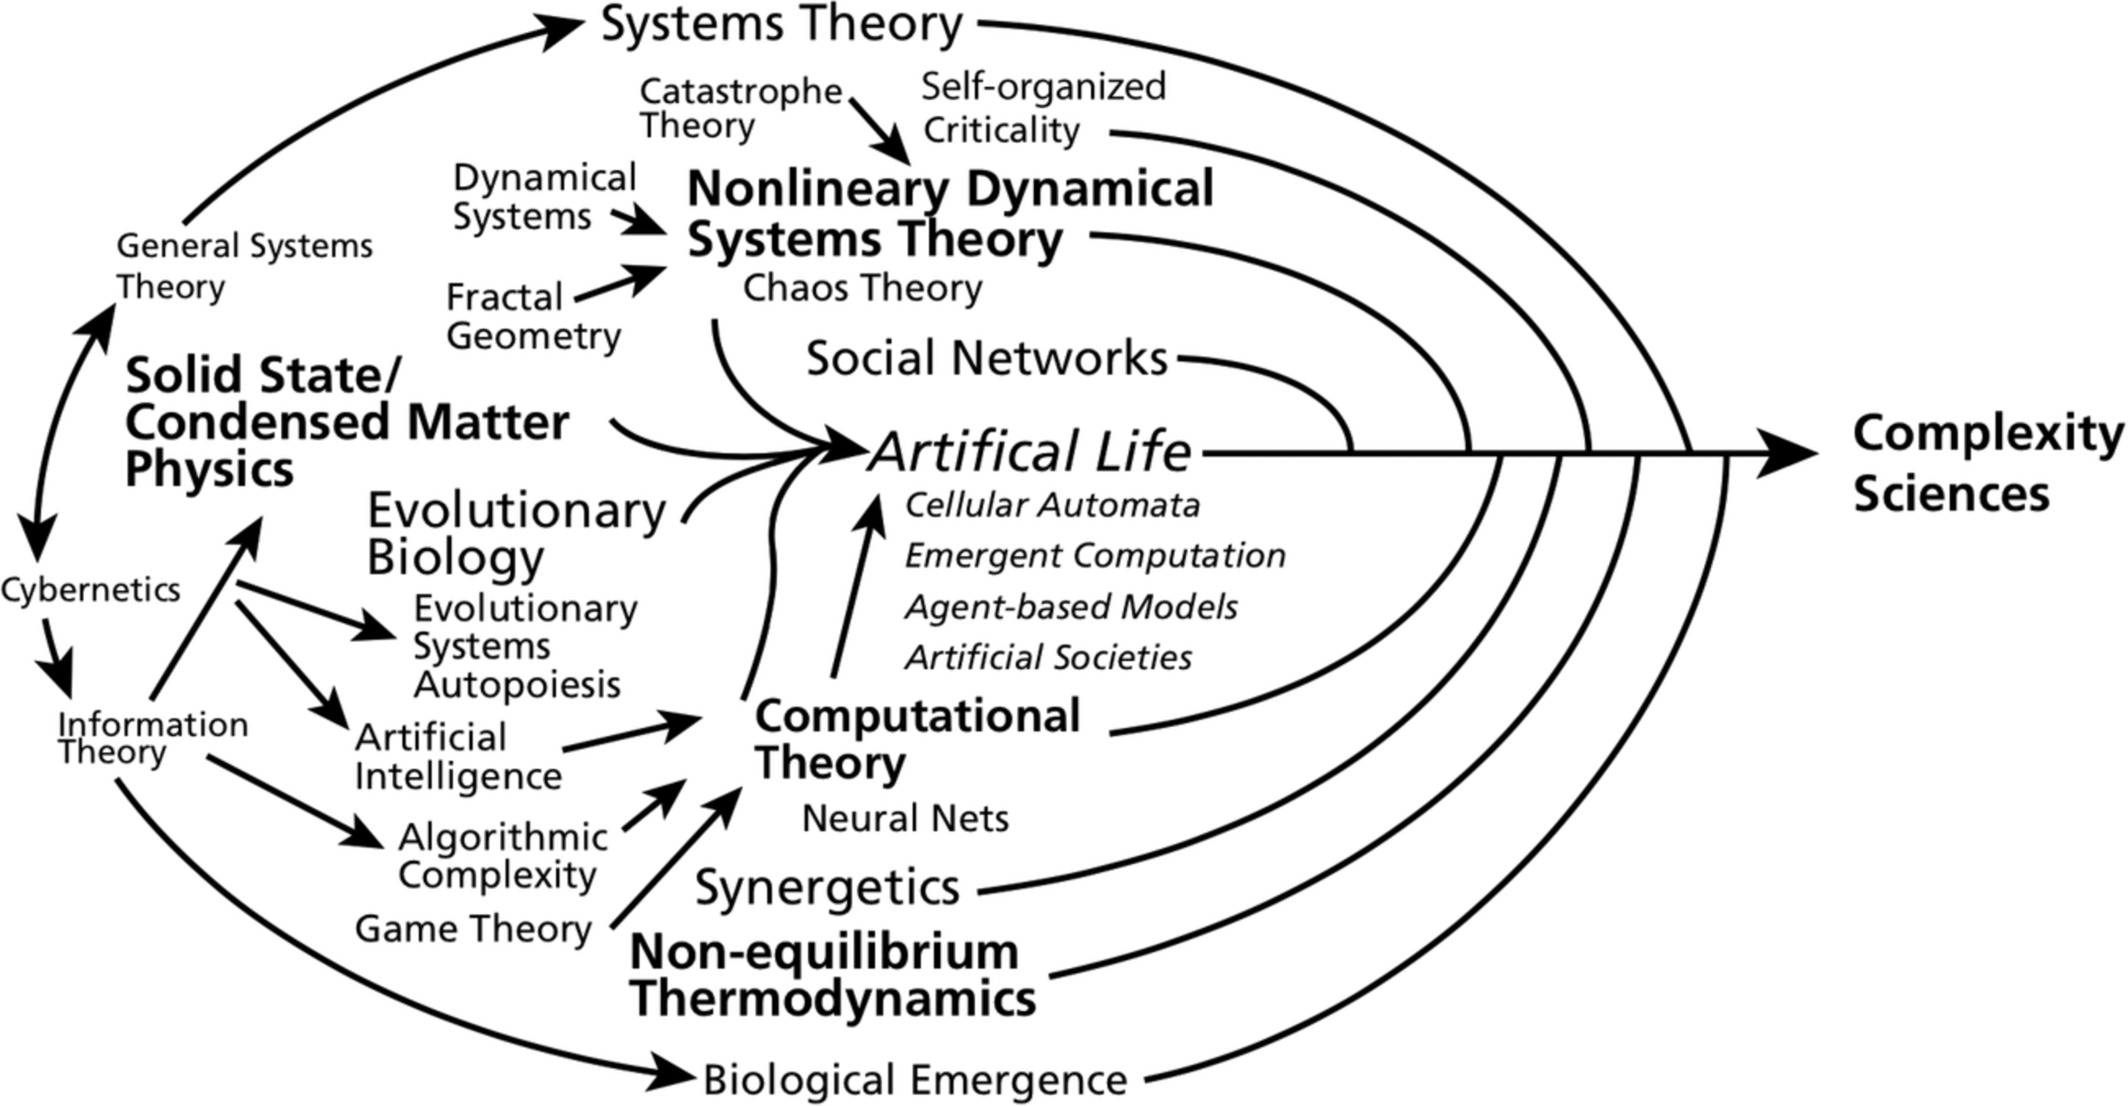
\includegraphics[keepaspectratio]{../include/img/wcs1525-fig-0001-m.jpg}}

}

\caption{Favela (2020) Figure 1}

\end{figure}%

\subsection{Levels of analysis}\label{levels-of-analysis}

\begin{figure}[H]

{\centering \pandocbounded{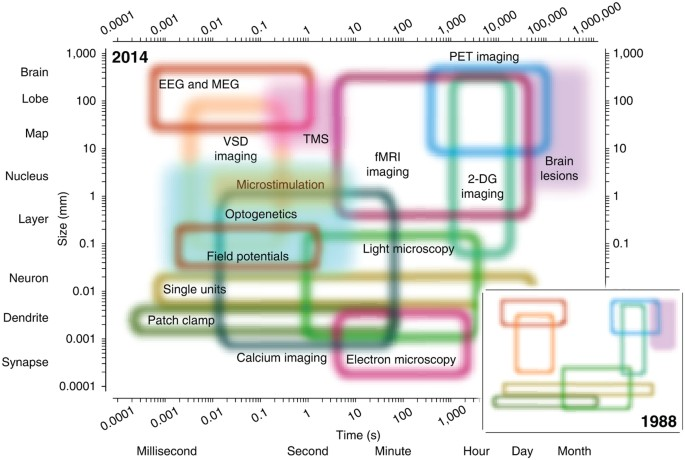
\includegraphics[keepaspectratio]{wk01-2025-01-16_files/mediabag/41593_2014_Article_B.jpg}}

}

\caption{Sejnowski et al. (2014) Figure 1}

\end{figure}%

\subsection{David Marr (1945-1980)}\label{david-marr-1945-1980}

\begin{figure}[H]

{\centering \pandocbounded{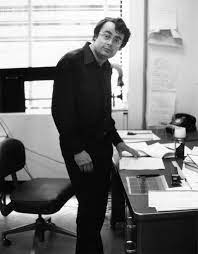
\includegraphics[keepaspectratio]{wk01-2025-01-16_files/mediabag/images-q=tbn-ANd9GcT.jpg}}

}

\caption{David Marr}

\end{figure}%

\begin{figure}[H]

{\centering \pandocbounded{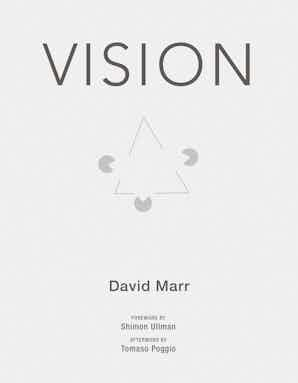
\includegraphics[keepaspectratio]{wk01-2025-01-16_files/mediabag/9780262514620.jpg}}

}

\caption{Marr (1980)}

\end{figure}%

\subsection{Marr's Three Levels}\label{marrs-three-levels}

\begin{figure}[H]

{\centering \pandocbounded{\includegraphics[keepaspectratio]{wk01-2025-01-16_files/mediabag/wcs1525-fig-0003-m.jpg}}

}

\caption{Favela (2020) Figure 3}

\end{figure}%

\begin{center}\rule{0.5\linewidth}{0.5pt}\end{center}

\begin{itemize}
\tightlist
\item
  What must be computed to carry out task X?
\item
  What algorithm is used to carry out the computation?
\item
  What hardware implements the algorithm?
\end{itemize}

\subsection{Computational level}\label{computational-level}

\begin{itemize}
\tightlist
\item
  What has to be computed?

  \begin{itemize}
  \tightlist
  \item
    What is the shape/form of that unknown object?
  \item
    What did that person just say?
  \item
    Is that unknown object a threat to me?
  \end{itemize}
\end{itemize}

\subsection{Algorithmic level}\label{algorithmic-level}

\begin{itemize}
\tightlist
\item
  What's the `recipe' for\ldots{}

  \begin{itemize}
  \tightlist
  \item
    computing shape
  \item
    perceiving speech
  \item
    recognizing threats
  \end{itemize}
\end{itemize}

\subsection{Implementation level}\label{implementation-level}

\begin{itemize}
\tightlist
\item
  How do\ldots{}

  \begin{itemize}
  \tightlist
  \item
    neurons
  \item
    areas
  \item
    networks
  \end{itemize}
\item
  implement the recipe?
\end{itemize}

\subsection{Causality in neuroscience}\label{causality-in-neuroscience}

\begin{itemize}
\tightlist
\item
  Siddiqi, Kording, Parvizi, \& Fox (2022)
\item
  Stimulation \& lesion studies needed for inferring \emph{causation}.
\item
  Bradford-Hill criteria (Hill, 2015)
\end{itemize}

\subsection{Varied notions of
mechanism}\label{varied-notions-of-mechanism}

\begin{figure}[H]

{\centering \pandocbounded{\includegraphics[keepaspectratio]{wk01-2025-01-16_files/mediabag/41583_2023_778_Fig1_.webp}}

}

\caption{Fig. 1: The narrow and broad notions of mechanism from Ross \&
Bassett (2024)}

\end{figure}%

\subsection{Toward reverse
neuroethology}\label{toward-reverse-neuroethology}

\begin{figure}[H]

{\centering \pandocbounded{\includegraphics[keepaspectratio]{wk01-2025-01-16_files/mediabag/ne470369.f1.gif}}

}

\caption{Figure 1 from Asinof \& Card (2024)}

\end{figure}%

\begin{center}\rule{0.5\linewidth}{0.5pt}\end{center}

\begin{figure}[H]

{\centering \pandocbounded{\includegraphics[keepaspectratio]{wk01-2025-01-16_files/mediabag/giphy.gif}}

}

\caption{https://giphy.com/clips/thefastsaga-fast-and-furious-saga-fate-of-the-DF34cUyak7TPs7D4GE}

\end{figure}%

\begin{center}\rule{0.5\linewidth}{0.5pt}\end{center}

\begin{quote}
\ldots when faced with a difficult question, we often answer an easier
one instead, usually without noticing the substitution.
\end{quote}

Kahneman (2013), p.~12 quoted in Krakauer, Ghazanfar, Gomez-Marin,
MacIver, \& Poeppel (2017)

\section{Break}\label{break}

\section{Your turn}\label{your-turn}

\subsection{Does neuroscience need
behavior?}\label{does-neuroscience-need-behavior}

Krakauer, J. W., Ghazanfar, A. A., Gomez-Marin, A., MacIver, M. A., \&
Poeppel, D. (2017). Neuroscience needs behavior: Correcting a
reductionist bias. \emph{Neuron}, \emph{93}(3), 480--490.
\url{https://dx.doi.org/10.1016/j.neuron.2016.12.041}.

Parada, F. J. \& Rossi, A. (2018). If neuroscience needs behavior, what
does psychology need? \emph{Frontiers in Psychology}, \emph{9}, 433.
\url{https://doi.org/10.3389/fpsyg.2018.00433}.

\subsection{Key points}\label{key-points}

\begin{itemize}
\tightlist
\item
  Questions `often tacit\ldots belief in the reductionist program for
  understanding the link between brain and behavior'
\item
  Behavior -\textgreater{} understanding; neural interventions
  -\textgreater{} causality
\item
  Marr's 3 levels (computation; algorithm; implementation)
\end{itemize}

\subsection{But what is behavior?}\label{but-what-is-behavior}

\subsection{``Behavioural biologists don't agree on what constitutes
behaviour''}\label{behavioural-biologists-dont-agree-on-what-constitutes-behaviour-1}

\begin{quote}
\ldots{}``Behaviour is the internally coordinated responses (actions or
inactions) of whole living organisms (individuals or groups) to internal
and/or external stimuli, excluding responses more easily understood as
developmental changes.''
\end{quote}

(Levitis et al., 2009)

\begin{center}\rule{0.5\linewidth}{0.5pt}\end{center}

\begin{figure}[H]

{\centering \pandocbounded{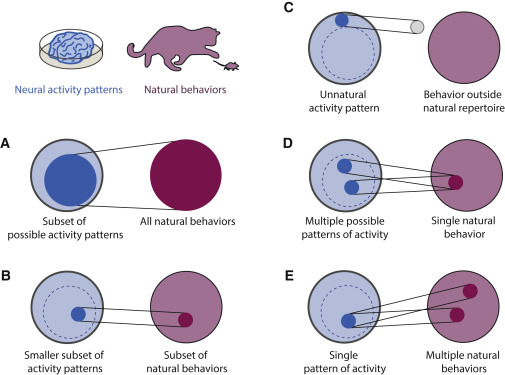
\includegraphics[keepaspectratio]{wk01-2025-01-16_files/mediabag/1-s2.0-S089662731631.jpg}}

}

\caption{(Krakauer et al., 2017, fig. 1)}

\end{figure}%

\begin{center}\rule{0.5\linewidth}{0.5pt}\end{center}

\begin{figure}[H]

{\centering \pandocbounded{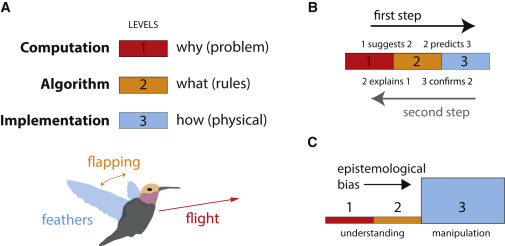
\includegraphics[keepaspectratio]{wk01-2025-01-16_files/mediabag/1-s2.0-S0896627316311.jpg}}

}

\caption{(Krakauer et al., 2017, fig. 2)}

\end{figure}%

\begin{center}\rule{0.5\linewidth}{0.5pt}\end{center}

\begin{figure}[H]

{\centering \pandocbounded{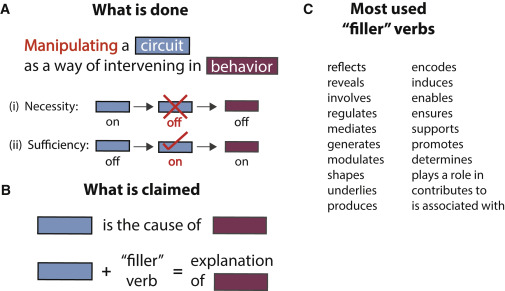
\includegraphics[keepaspectratio]{wk01-2025-01-16_files/mediabag/1-s2.0-S08966273163112.jpg}}

}

\caption{(Krakauer et al., 2017, fig. 3)}

\end{figure}%

\begin{center}\rule{0.5\linewidth}{0.5pt}\end{center}

\begin{figure}[H]

{\centering \pandocbounded{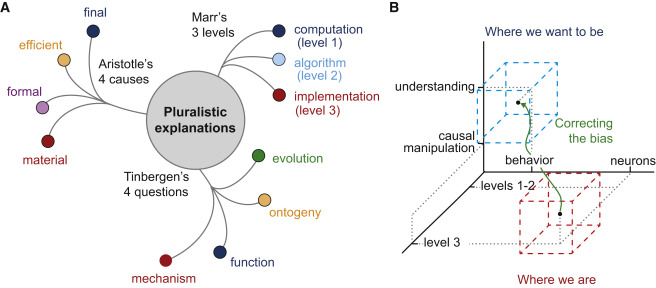
\includegraphics[keepaspectratio]{wk01-2025-01-16_files/mediabag/1-s2.0-S089662731631123.jpg}}

}

\caption{(Krakauer et al., 2017, fig. 4)}

\end{figure}%

\begin{center}\rule{0.5\linewidth}{0.5pt}\end{center}

\begin{figure}[H]

{\centering \pandocbounded{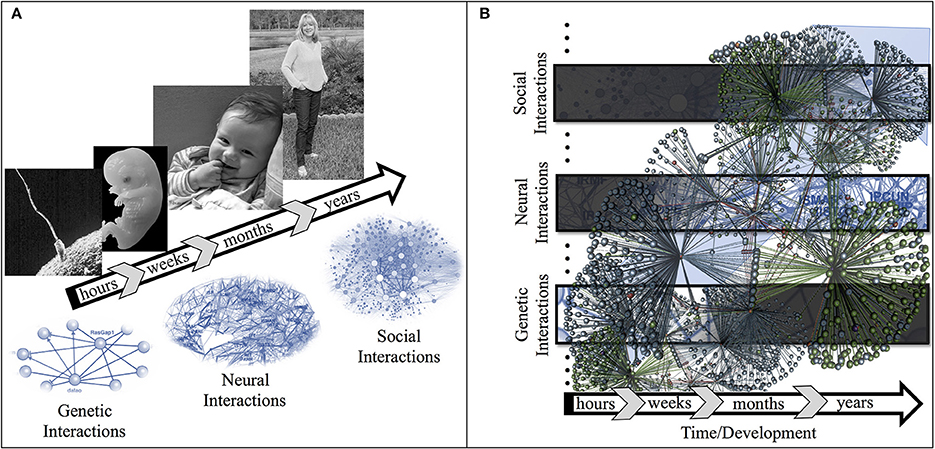
\includegraphics[keepaspectratio]{wk01-2025-01-16_files/mediabag/fpsyg-09-00433-g001.jpg}}

}

\caption{(Parada \& Rossi, 2018, fig. 1)}

\end{figure}%

\subsection{Exercise 01}\label{exercise-01}

\begin{itemize}
\tightlist
\item
  {\href{../exercises/ex01.qmd}{Due next Wednesday}}
\end{itemize}

\subsection{Main points}\label{main-points}

\begin{itemize}
\tightlist
\item
  Psychology is harder than physics
\item
  Neuroscience needs behavior
\item
  Psychology needs behavior + mental states + measures of environment
\end{itemize}

\subsection{Next time\ldots{}}\label{next-time}

\begin{itemize}
\tightlist
\item
  Neuroanatomy lab

  \begin{itemize}
  \tightlist
  \item
    Read/study

    \begin{itemize}
    \tightlist
    \item
      Neuroanatomy \href{../resources/anatomy.qmd}{notes}
    \item
      Bring to class a copy of \href{exercises/ex02.pdf}{Exercise 02}
    \end{itemize}
  \end{itemize}
\end{itemize}

\section{Resources}\label{resources}

\subsection*{References}\label{references}
\addcontentsline{toc}{subsection}{References}

\phantomsection\label{refs}
\begin{CSLReferences}{1}{0}
\bibitem[\citeproctext]{ref-Asinof2024-iu}
Asinof, S. K., \& Card, G. M. (2024). Neural control of naturalistic
behavior choices. \emph{Annual Review of Neuroscience}, \emph{47},
369--388. \url{https://doi.org/10.1146/annurev-neuro-111020-094019}

\bibitem[\citeproctext]{ref-Becker2021-bd}
Becker, C. R. (2021, August 31). A comprehensive list of human-computer
interactions. Retrieved January 8, 2025, from
\url{https://uxdesign.cc/a-comprehensive-list-of-human-computer-interactions-d72eaca2c0df}

\bibitem[\citeproctext]{ref-Calabrese2018-ve}
Calabrese, R. L. (2018). Inconvenient truth to principle of
neuroscience. \emph{Trends in Neurosciences}, \emph{41}(8), 488--491.
\url{https://doi.org/10.1016/j.tins.2018.05.006}

\bibitem[\citeproctext]{ref-Cepelewicz2021-hq}
Cepelewicz, J. (2021, August). Mental phenomena don't map into the brain
as expected.
\url{https://www.quantamagazine.org/mental-phenomena-dont-map-into-the-brain-as-expected-20210824/}.
Retrieved from
\url{https://www.quantamagazine.org/mental-phenomena-dont-map-into-the-brain-as-expected-20210824/}

\bibitem[\citeproctext]{ref-Cisek2019-vq}
Cisek, P. (2019). Resynthesizing behavior through phylogenetic
refinement. \emph{Attention, Perception \& Psychophysics}.
\url{https://doi.org/10.3758/s13414-019-01760-1}

\bibitem[\citeproctext]{ref-Eisenberg2019-iy}
Eisenberg, I. W., Bissett, P. G., Zeynep Enkavi, A., Li, J., MacKinnon,
D. P., Marsch, L. A., \& Poldrack, R. A. (2019). Uncovering the
structure of self-regulation through data-driven ontology discovery.
\emph{Nature Communications}, \emph{10}(1), 2319.
\url{https://doi.org/10.1038/s41467-019-10301-1}

\bibitem[\citeproctext]{ref-Favela2020-uc}
Favela, L. H. (2020). Cognitive science as complexity science.
\emph{Wiley Interdisciplinary Reviews. Cognitive Science}, \emph{11}(4),
e1525. \url{https://doi.org/10.1002/wcs.1525}

\bibitem[\citeproctext]{ref-Gilmore2016-lq}
Gilmore, R. O., Thomas, A. L., \& Fesi, J. (2016). Children's brain
responses to optic flow vary by pattern type and motion speed.
\emph{PloS One}, \emph{11}, e0157911.
\url{https://doi.org/10.1371/journal.pone.0157911}

\bibitem[\citeproctext]{ref-Hill2015-jb}
Hill, A. B. (2015). The environment and disease: Association or
causation? 1965. \emph{Journal of the Royal Society of Medicine},
\emph{108}(1), 32--37. \url{https://doi.org/10.1177/0141076814562718}

\bibitem[\citeproctext]{ref-Kahneman2013-zi}
Kahneman, D. (2013). \emph{Thinking, fast and slow} (1st edition).
Farrar, Straus; Giroux. Retrieved from
\url{https://www.amazon.com/Thinking-Fast-Slow-Daniel-Kahneman/dp/0374533555}

\bibitem[\citeproctext]{ref-Krakauer2017-xl}
Krakauer, J. W., Ghazanfar, A. A., Gomez-Marin, A., MacIver, M. A., \&
Poeppel, D. (2017). Neuroscience needs behavior: Correcting a
reductionist bias. \emph{Neuron}, \emph{93}(3), 480--490.
\url{https://doi.org/10.1016/j.neuron.2016.12.041}

\bibitem[\citeproctext]{ref-Levitis2009-br}
Levitis, D. A., Lidicker, W. Z., \& Freund, G. (2009). Behavioural
biologists don't agree on what constitutes behaviour. \emph{Animal
Behaviour}, \emph{78}(1), 103--110.
\url{https://doi.org/10.1016/j.anbehav.2009.03.018}

\bibitem[\citeproctext]{ref-Marr1980-cu}
Marr, D. (1980). \emph{Vision}. Retrieved from
\url{https://mitpress.mit.edu/books/vision}

\bibitem[\citeproctext]{ref-Melodysheep2011-wg}
melodysheep. (2011, March). Ode to the brain! By symphony of science.
Youtube. Retrieved from
\url{https://www.youtube.com/watch?v=JB7jSFeVz1U}

\bibitem[\citeproctext]{ref-National_Geographic2014-gv}
National Geographic. (2014, January). Beautiful {3-D} brain scans show
every synapse \textbar{} national geographic. You{T}ube. Retrieved from
\url{https://www.youtube.com/watch?v=nvXuq9jRWKE}

\bibitem[\citeproctext]{ref-Parada2018-rp}
Parada, F. J., \& Rossi, A. (2018). If neuroscience needs behavior, what
does psychology need? \emph{Frontiers in Psychology}, \emph{9}, 433.
\url{https://doi.org/10.3389/fpsyg.2018.00433}

\bibitem[\citeproctext]{ref-Qian2022-yp}
Qian, Y., Berenbaum, S. A., \& Gilmore, R. O. (2022). Vision contributes
to sex differences in spatial cognition and activity interests.
\emph{Scientific Reports}, \emph{12}, 17623.
\url{https://doi.org/10.1038/s41598-022-22269-y}

\bibitem[\citeproctext]{ref-Ross2024-nr}
Ross, L. N., \& Bassett, D. S. (2024). Causation in neuroscience:
Keeping mechanism meaningful. \emph{Nature Reviews. Neuroscience}.
\url{https://doi.org/10.1038/s41583-023-00778-7}

\bibitem[\citeproctext]{ref-Segal2024-ht}
Segal, A., Tiego, J., Parkes, L., Holmes, A. J., Marquand, A. F., \&
Fornito, A. (2024). Embracing variability in the search for biological
mechanisms of psychiatric illness. \emph{Trends in Cognitive Sciences},
\emph{29}, 85--99. \url{https://doi.org/10.1016/j.tics.2024.09.010}

\bibitem[\citeproctext]{ref-Sejnowski2014-aa}
Sejnowski, T. J., Churchland, P. S., \& Movshon, J. A. (2014). Putting
big data to good use in neuroscience. \emph{Nat. Neurosci.},
\emph{17}(11), 1440--1441. \url{https://doi.org/10.1038/nn.3839}

\bibitem[\citeproctext]{ref-Siddiqi2022-wl}
Siddiqi, S. H., Kording, K. P., Parvizi, J., \& Fox, M. D. (2022).
Causal mapping of human brain function. \emph{Nature {R}eviews
{N}euroscience}, \emph{23}(6), 361--375.
\url{https://doi.org/10.1038/s41583-022-00583-8}

\bibitem[\citeproctext]{ref-Stringer2019-vf}
Stringer, C., Pachitariu, M., Steinmetz, N., Reddy, C. B., Carandini,
M., \& Harris, K. D. (2019). Spontaneous behaviors drive
multidimensional, brainwide activity. \emph{Science}, \emph{364}(6437),
255. \url{https://doi.org/10.1126/science.aav7893}

\bibitem[\citeproctext]{ref-swanson2005anatomy}
Swanson, L. W. (2005). Anatomy of the soul as reflected in the cerebral
hemispheres: Neural circuits underlying voluntary control of basic
motivated behaviors. \emph{Journal of Comparative Neurology},
\emph{493}(1), 122--131. \url{https://doi.org/10.1002/cne.20733}

\bibitem[\citeproctext]{ref-Swanson2016-qr}
Swanson, L. W., \& Lichtman, J. W. (2016). From {C}ajal to connectome
and beyond. \emph{Annual Review of Neuroscience}, \emph{39}, 197--216.
\url{https://doi.org/10.1146/annurev-neuro-071714-033954}

\end{CSLReferences}




\end{document}
